\documentclass[12pt]{paper}
%\usepackage{paper} %if the document does not compile properly for you on the initial build, uncomment \usepackage{paper} and build again. This should force MikTeX to install package "paper"
\usepackage[margin=1in]{geometry}
\usepackage{float}
\usepackage{natbib}
\bibliographystyle{apsr}
\usepackage{graphicx}
\graphicspath{ {../fig/} }
\usepackage{setspace}
\usepackage[super]{nth}
\usepackage{booktabs}
\usepackage{makecell}
\usepackage{amsmath}
\usepackage{dcolumn}
%\usepackage{authblk}
\usepackage{hyperref}
\usepackage{wrapfig}
%\usepackage{etoolbox}
%
%\AtBeginEnvironment{quote}{\singlespacing\small}
\usepackage{epigraph}
%"In New York, it isn't between Democrat and Republican, it's between top and down"
\begin{document}

\title{Not Homogeneous: Intra-party affect}
\author{Robert Lytle}
\date{\today}
\maketitle
\epigraph{This is not the Republicans vs the Democrats---this is the elites of the Republican and Democratic party who have driven this country into the ditch vs Donald J. Trump and the Rest of America.}{\textit{Roger Stone %(Get Me Roger Stone)
}}
\epigraph{Establishment power in Washington is not always centered around left versus right. Often, it’s about up versus down.}{\textit{Alexandria Ocasio-Cortez}}
%\epigraph{The beauty of the tea party movement is that it is independent and thus a true check and balance of the Republican and Democrat parties. It's not a pawn of the GOP, thus untouchable in criticism of the Democrats---I view it as an unattached conscience of the Republican party.}{\textit{Dana Loesch}}
\setstretch{2}
%\thispagestyle{empty}
%\clearpage
%\setstretch{1}


%Previous studies of affective polarization (e.g. \citet{iyengar2012affect}) have  focused on partisans' net partisan affect, this approach is problematic. When using a measure built from both in party and out party evaluations, it is not clear whether a change in NPA is borne of a change in in-party or out-party feeling. For example, the mean out-party affect of Republicans and Democrats in 2016 were each about 25 (Figure \ref{fig:cdf-mean}), but Republicans' NPA was significantly lower than Democrats' (Figure \ref{fig:cdf-npa}). Ostensibly, Republicans were \textit{less} polarized than Democrats, but to say so belies the fact that Republicans are very cold towards Democrats, they are just somewhat colder towards \textit{their own} party as well.
%\begin{figure}[H]
%\center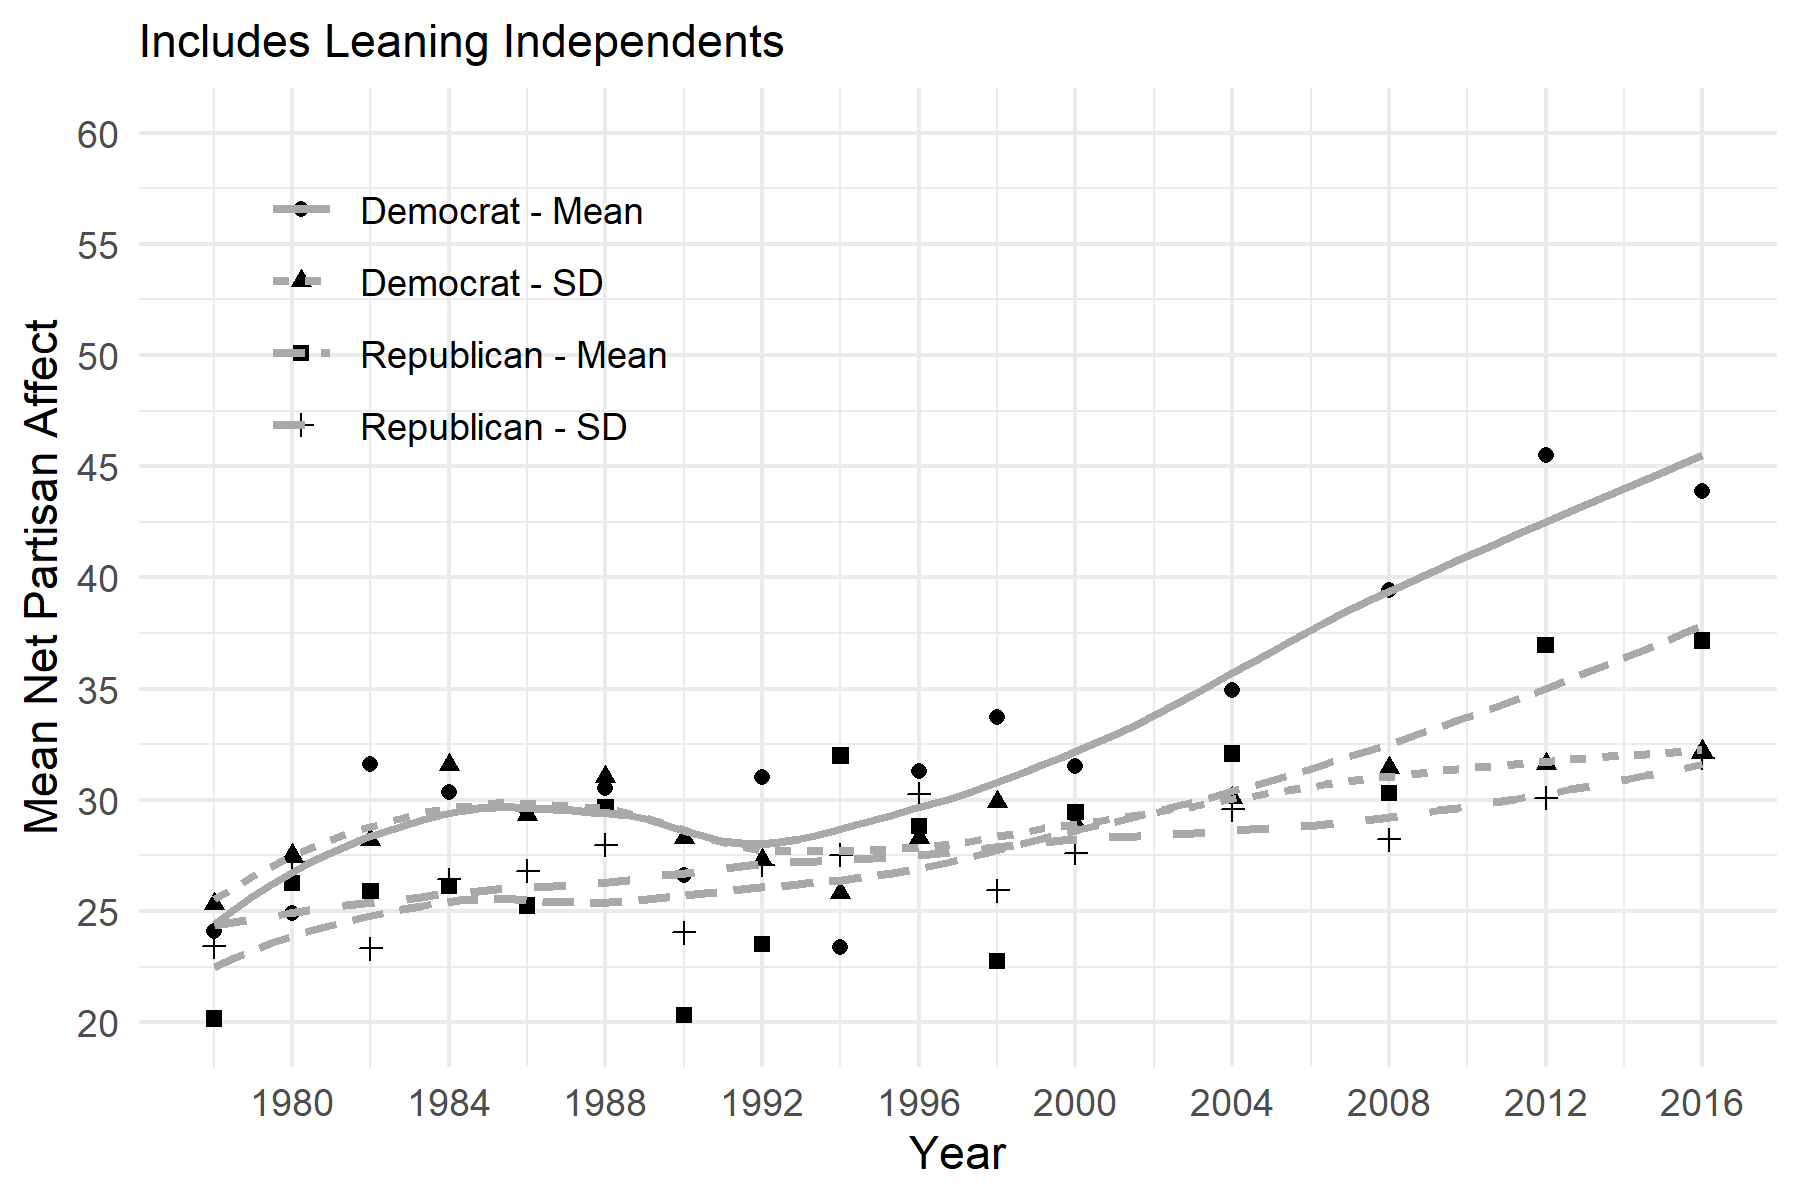
\includegraphics[width=5in]{cdf-npa-ns.png}
%\caption{\label{fig:cdf-npa} \textit{\textbf{Mean of Partisans' in-party and out-party feeling thermometers as reported in the ANES, 1978--2016.} Republicans tend to be colder in general.}}
%\end{figure}

\section{Introduction}
Affective and social distance between Democrats and Republicans has expanded dramatically. Scholars of affective polarization have largely considered partisans to be warm towards their parties and co-partisans and cold to members of the out party \citep{iyengar2012affect, iyengar2018strengthening}. These scholars argue that the ``Net Partisan Affect" of Democrats and Republicans---the


%Not super happy with "midst of disagreements"
Recent developments give us cause, however, to doubt the consistency of in-party warmth; Factions in both parties have received a great deal of attention in recent years. Groups like the Tea Party and alt-right in the Republican Party and progressives and socialists in the Democratic party have presented challenges to their party's status-quo, often acting in opposition to their party's elites [CITE]. In the midst of these in-party disagreements the 2016 and 2020 election cycles have been characterized by lengthy and contentious primary elections. There has been no shortage of media accounts describing chaos at party conventions [CITE] and increasingly salient divides between populist and establishment wings of both parties [CITE]. 

Using the 2016 Democratic primary \cite{wronski2018tale} demonstrate that Democrats in 2016 primary were divided along autoritarian lines. Primary voters scoring high in authoritarian personality traits were more likely to support Hillary Clinton---those with few authoritarian tendencies were likely to be supporters of Bernie Sanders. For example, \cite{iyengar2018strengthening} find that the strength of partisans' out-party animus has supplanted in-party warmth as a predictor of voting behavior. 

%Rohde (1991) elite heterogeneity decreases salience of party ID
%ask Dr. Bankert if okay to \cite{bankert2020authoritarian}


By focusing on mean in-party feeling---rather than the distribution of partisan affect---researchers paint too optimistic a view of partisanship's strength. My findings bolster those of  \cite{klar2018affective}---partisan warmth has declined across the board.

%When the dependent variable in studies of polarization includes by default feelings towards the in-party, it becomes impossible to study how the effects of in-party feelings themselves have changed over time, or even to determine if they have any effect at all.



\section{Data}

The data from this study were taken from the American National Election Study Cumulative Data File\footnote{https://electionstudies.org/data-center/anes-time-series-cumulative-data-file/}. All data and replication materials will be made available on GitHub. Some figures have been built using samples \textit{including} leaning partisans, while others \textit{exclude} leaning partisans, despite the evidence that partisan leaning independents behave in much the same way as their sorted counterparts \citep{klar2016independent}\footnote{The upper left corner of each figure indicates whether leaning independents were included in the sample.This will certainly change before the paper is finished, I've generated figs for both and have been going back and forth}. By restricting the sample to avowed partisans, I am likely underestimating the variation/animosity present in in-party attitudes, and overestimating the proportion of Democrat and Republican voters who are lukewarm or ambivalent towards their party. Regardless of the samples used, the topline finding is the same: \textbf{An increasing number of Democrats and Republicans, voters and nonvoters, and partisans and non-partisans are lukewarm or cold---not just towards an out-party but towards both major parties.}


\section{Results}

\begin{figure}[H]
\centering
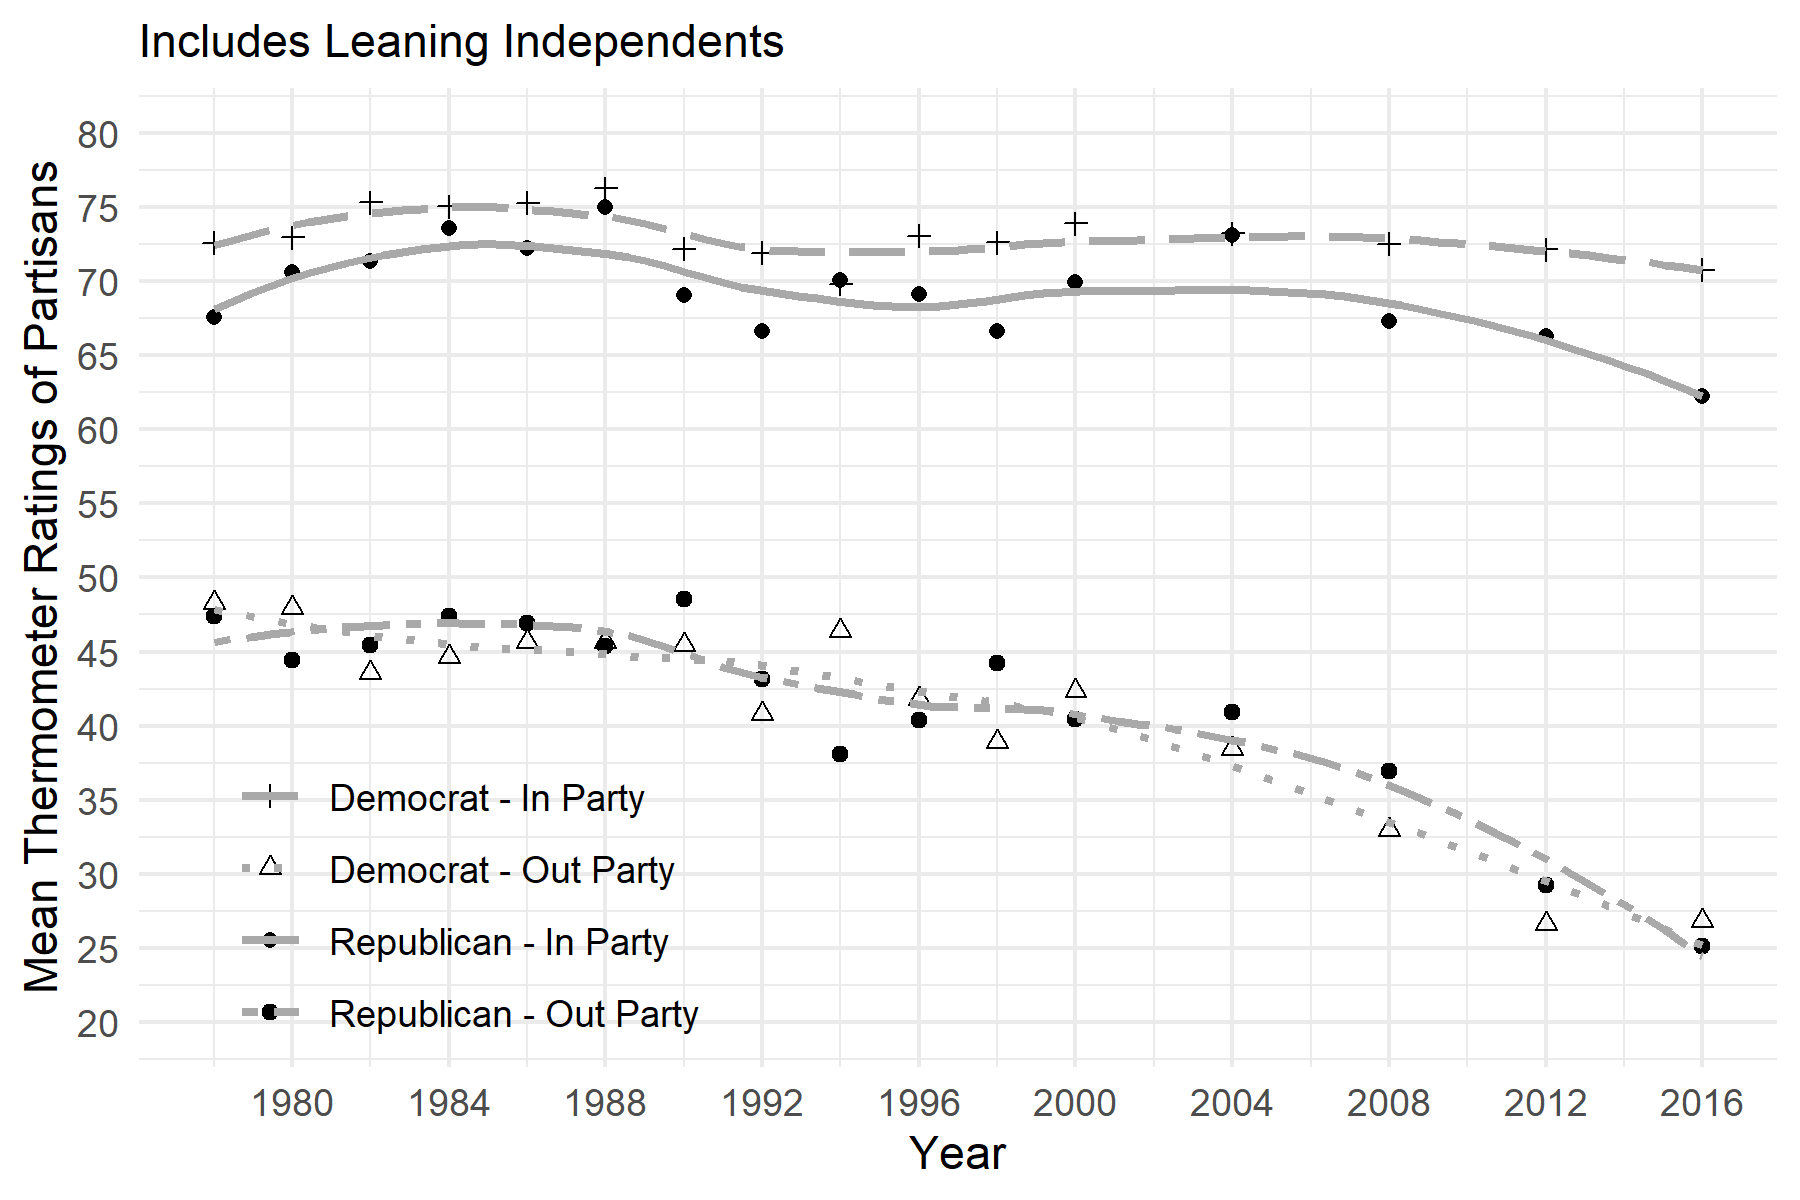
\includegraphics[width=.8\textwidth]{cdf-mean-ns.png}
\caption{\label{fig:cdf-mean} \textit{\textbf{Mean of Partisans' in-party and out-party feeling thermometers as reported in the ANES, 1978--2016.}% Republicans tend to be colder in general.
}}
\end{figure}
As shown in Figure \ref{fig:cdf-mean}, mean out party feeling thermometers for Democrats and Republicans have obviously declined. We also a see a decline in Republican's in party FTs since 2004, and only a slight decline in those of Democrats. Partisans remain much warmer (on average) towards their party than the opposition this---particularly in the case of Republicans---is in spite of a decline in average in-party FTs.

\begin{wrapfigure}{R}{.8\textwidth}
\centering
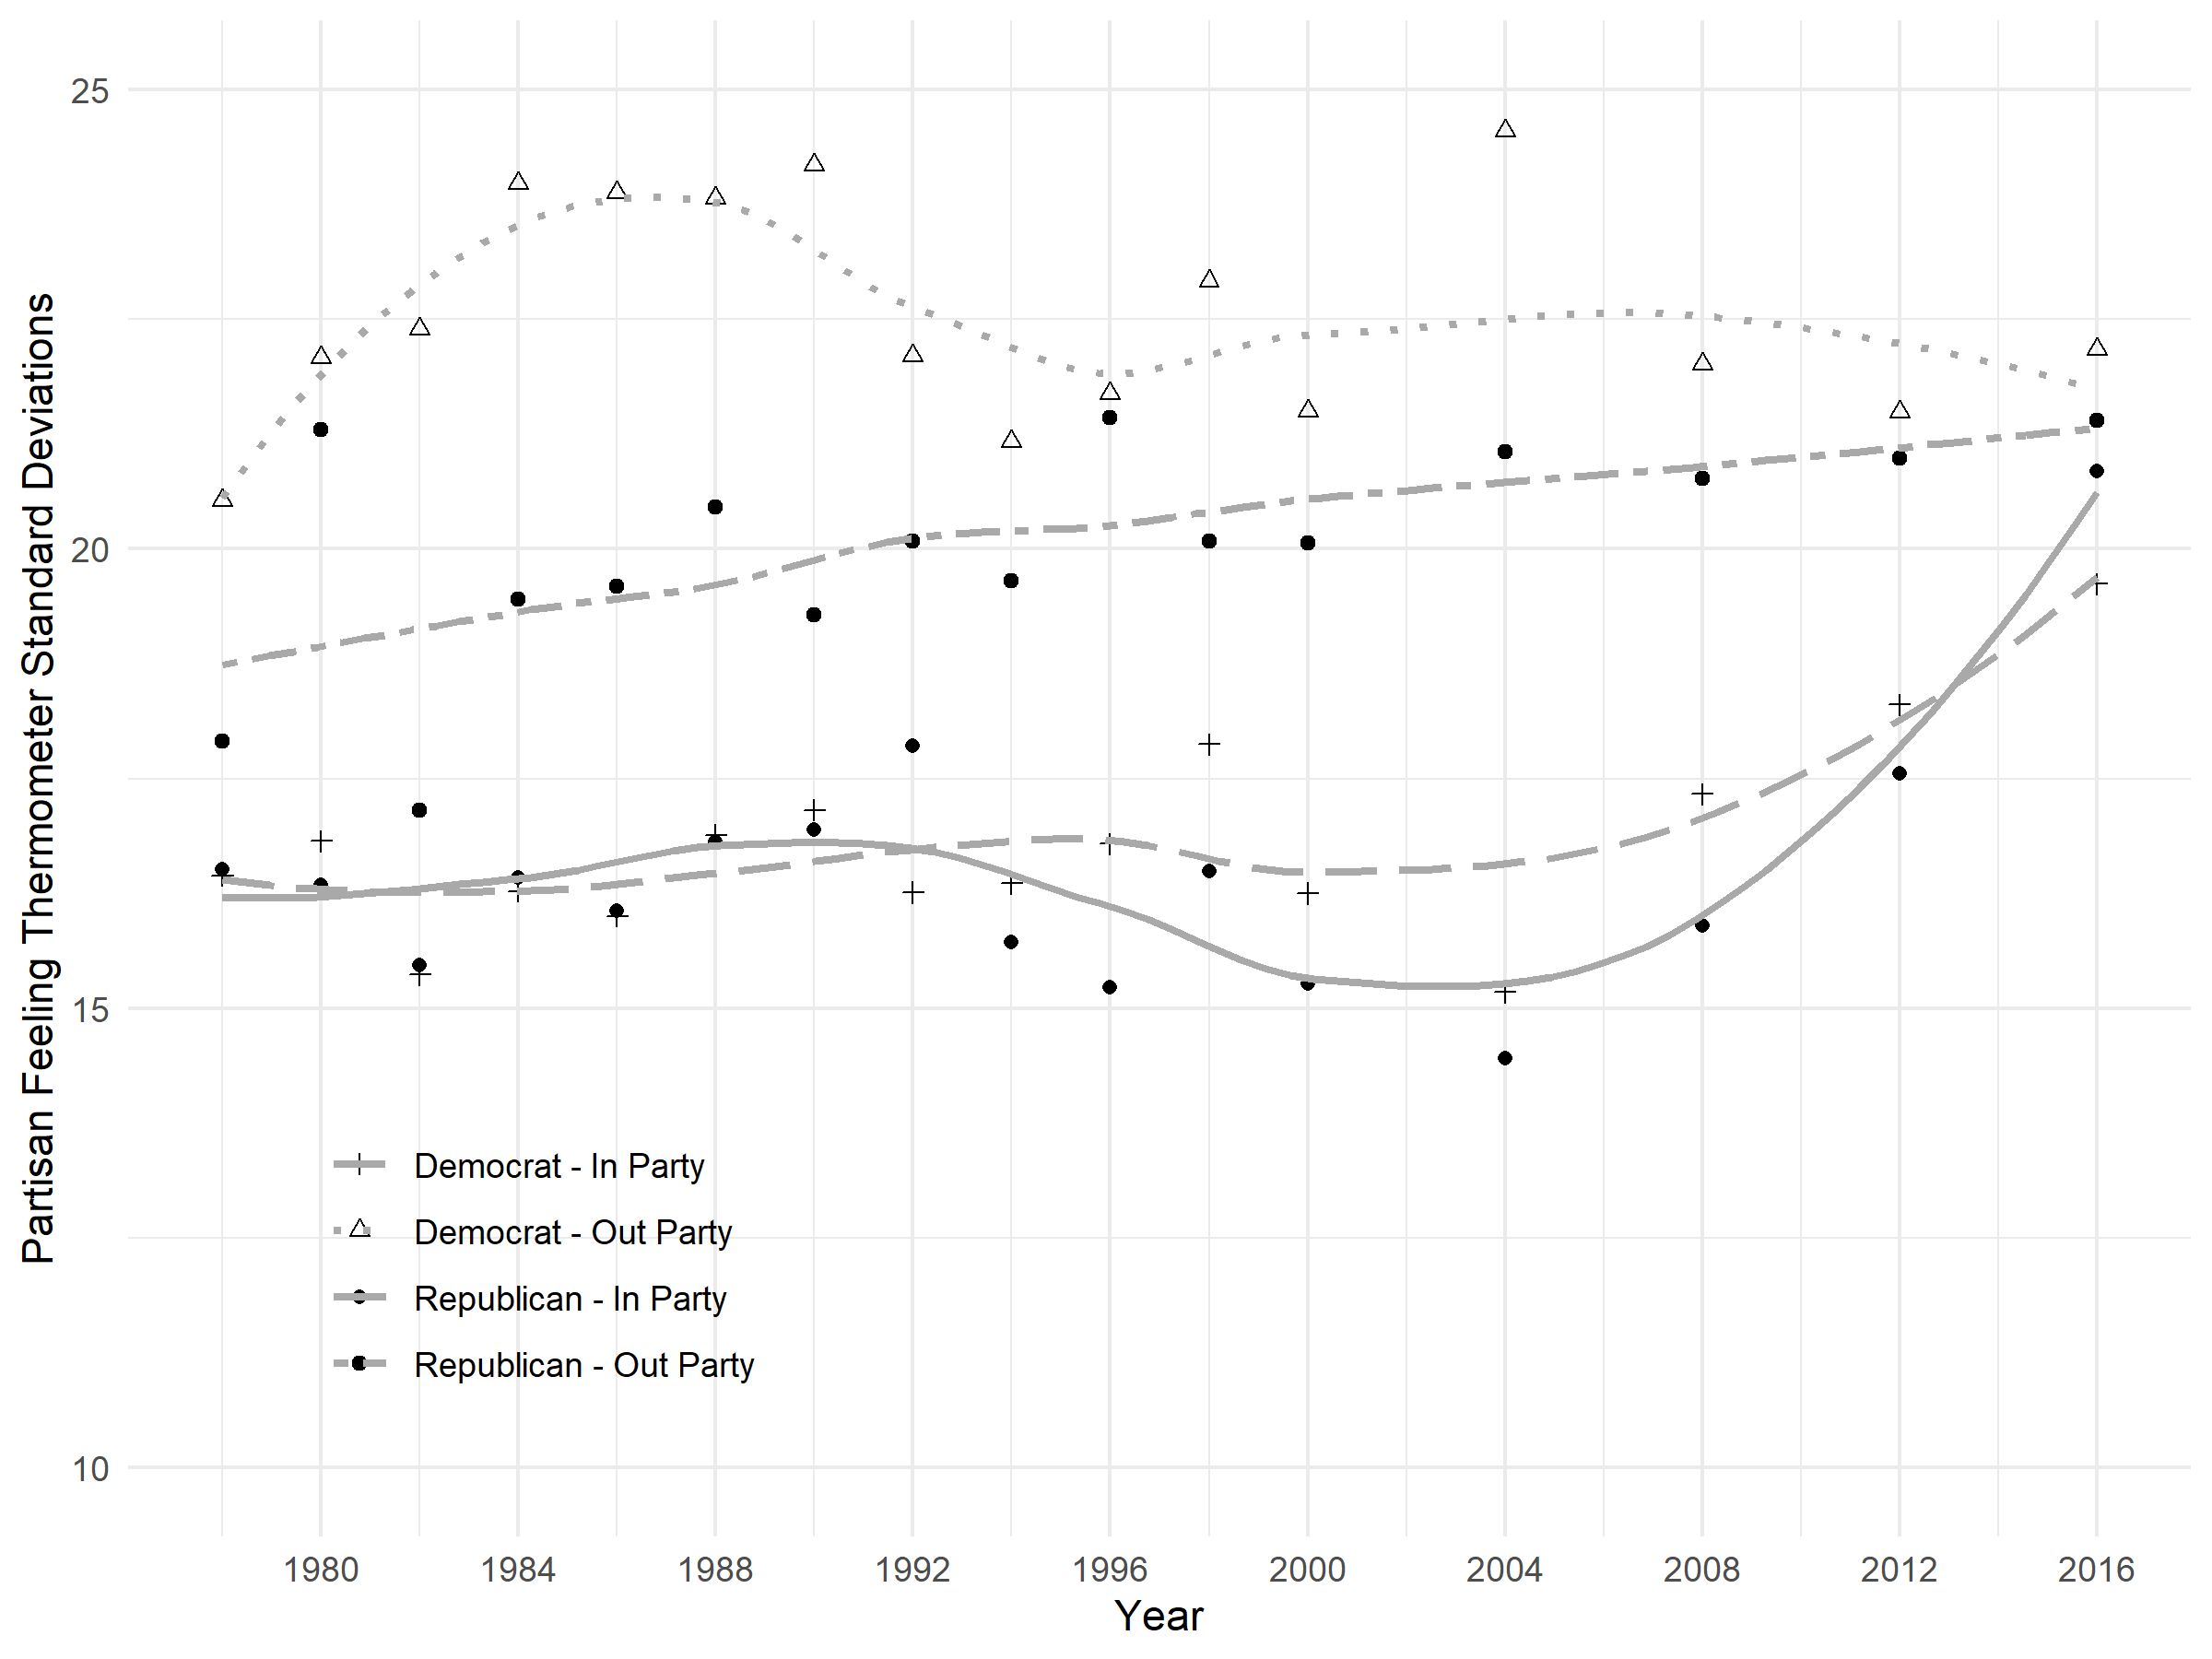
\includegraphics[width=.75\textwidth]{cdf-sd.png}
\caption{\label{fig:cdf-sd} \textit{\textbf{Standard Deviation of partisans' in party feeling thermometers as reported in the ANES, 1978--2016.} %After several decades of minimal change, the variation in in-party feeling thermometer ratings increased substantially between 2004 and 2016. This change is robust to both the Fligner-Killeen and Levene's tests of homogeneity of variance.
}}
\end{wrapfigure}

From 2004--2016 the variance of in-party Feeling thermometers has increased. the SD of Republicans' in-party FTs increased from 14--21 in this period, while Democrats' increased from 15--19. Alone, these numbers are not all that impressive, but as is made clear by Figure \ref{fig:cdf-sd}, an increase in variation of this magnitude has never before been observed, nor has the trend continued for so many years.

As variance increases, so to has the proportion of partisans who rate their own party below a 50---a substantively meaningful threshold indicating that partisans are more cold than warm toward their own party. When leaning independents are included (following \citep{klar2016independent}), 10\% of Democrats and almost 20\% of Republicans are found to be cold towards their own party (up from 5\% each in 2004), while a sample which excludes leaning independents indicates 13\% of Republicans and 8\% of Democrats to be cold. Regardless of the cut-off point used to indicate cold affect, or the strength of partisans' identification with their party, the trend is robust---more partisans were cold to their party than has been observed at any point across the available data.

Negative evaluations of parties are increasingly common. The modal value of independents' average party FT has always been 50; in the late \nth{20} century, the distribution was characterized by a rightward tail. From 2000--2016 that tail has shifted left. Far more independents now have a net-negative disposition towards the two major parties. Similarly, when examining the distributions of in-party feeling thermometers the left skew has become more apparent; more Republicans and Democrats are now cold---below 50---toward their party than at any point in the range of data.

\begin{wrapfigure}{L}{.7\textwidth}
\centering
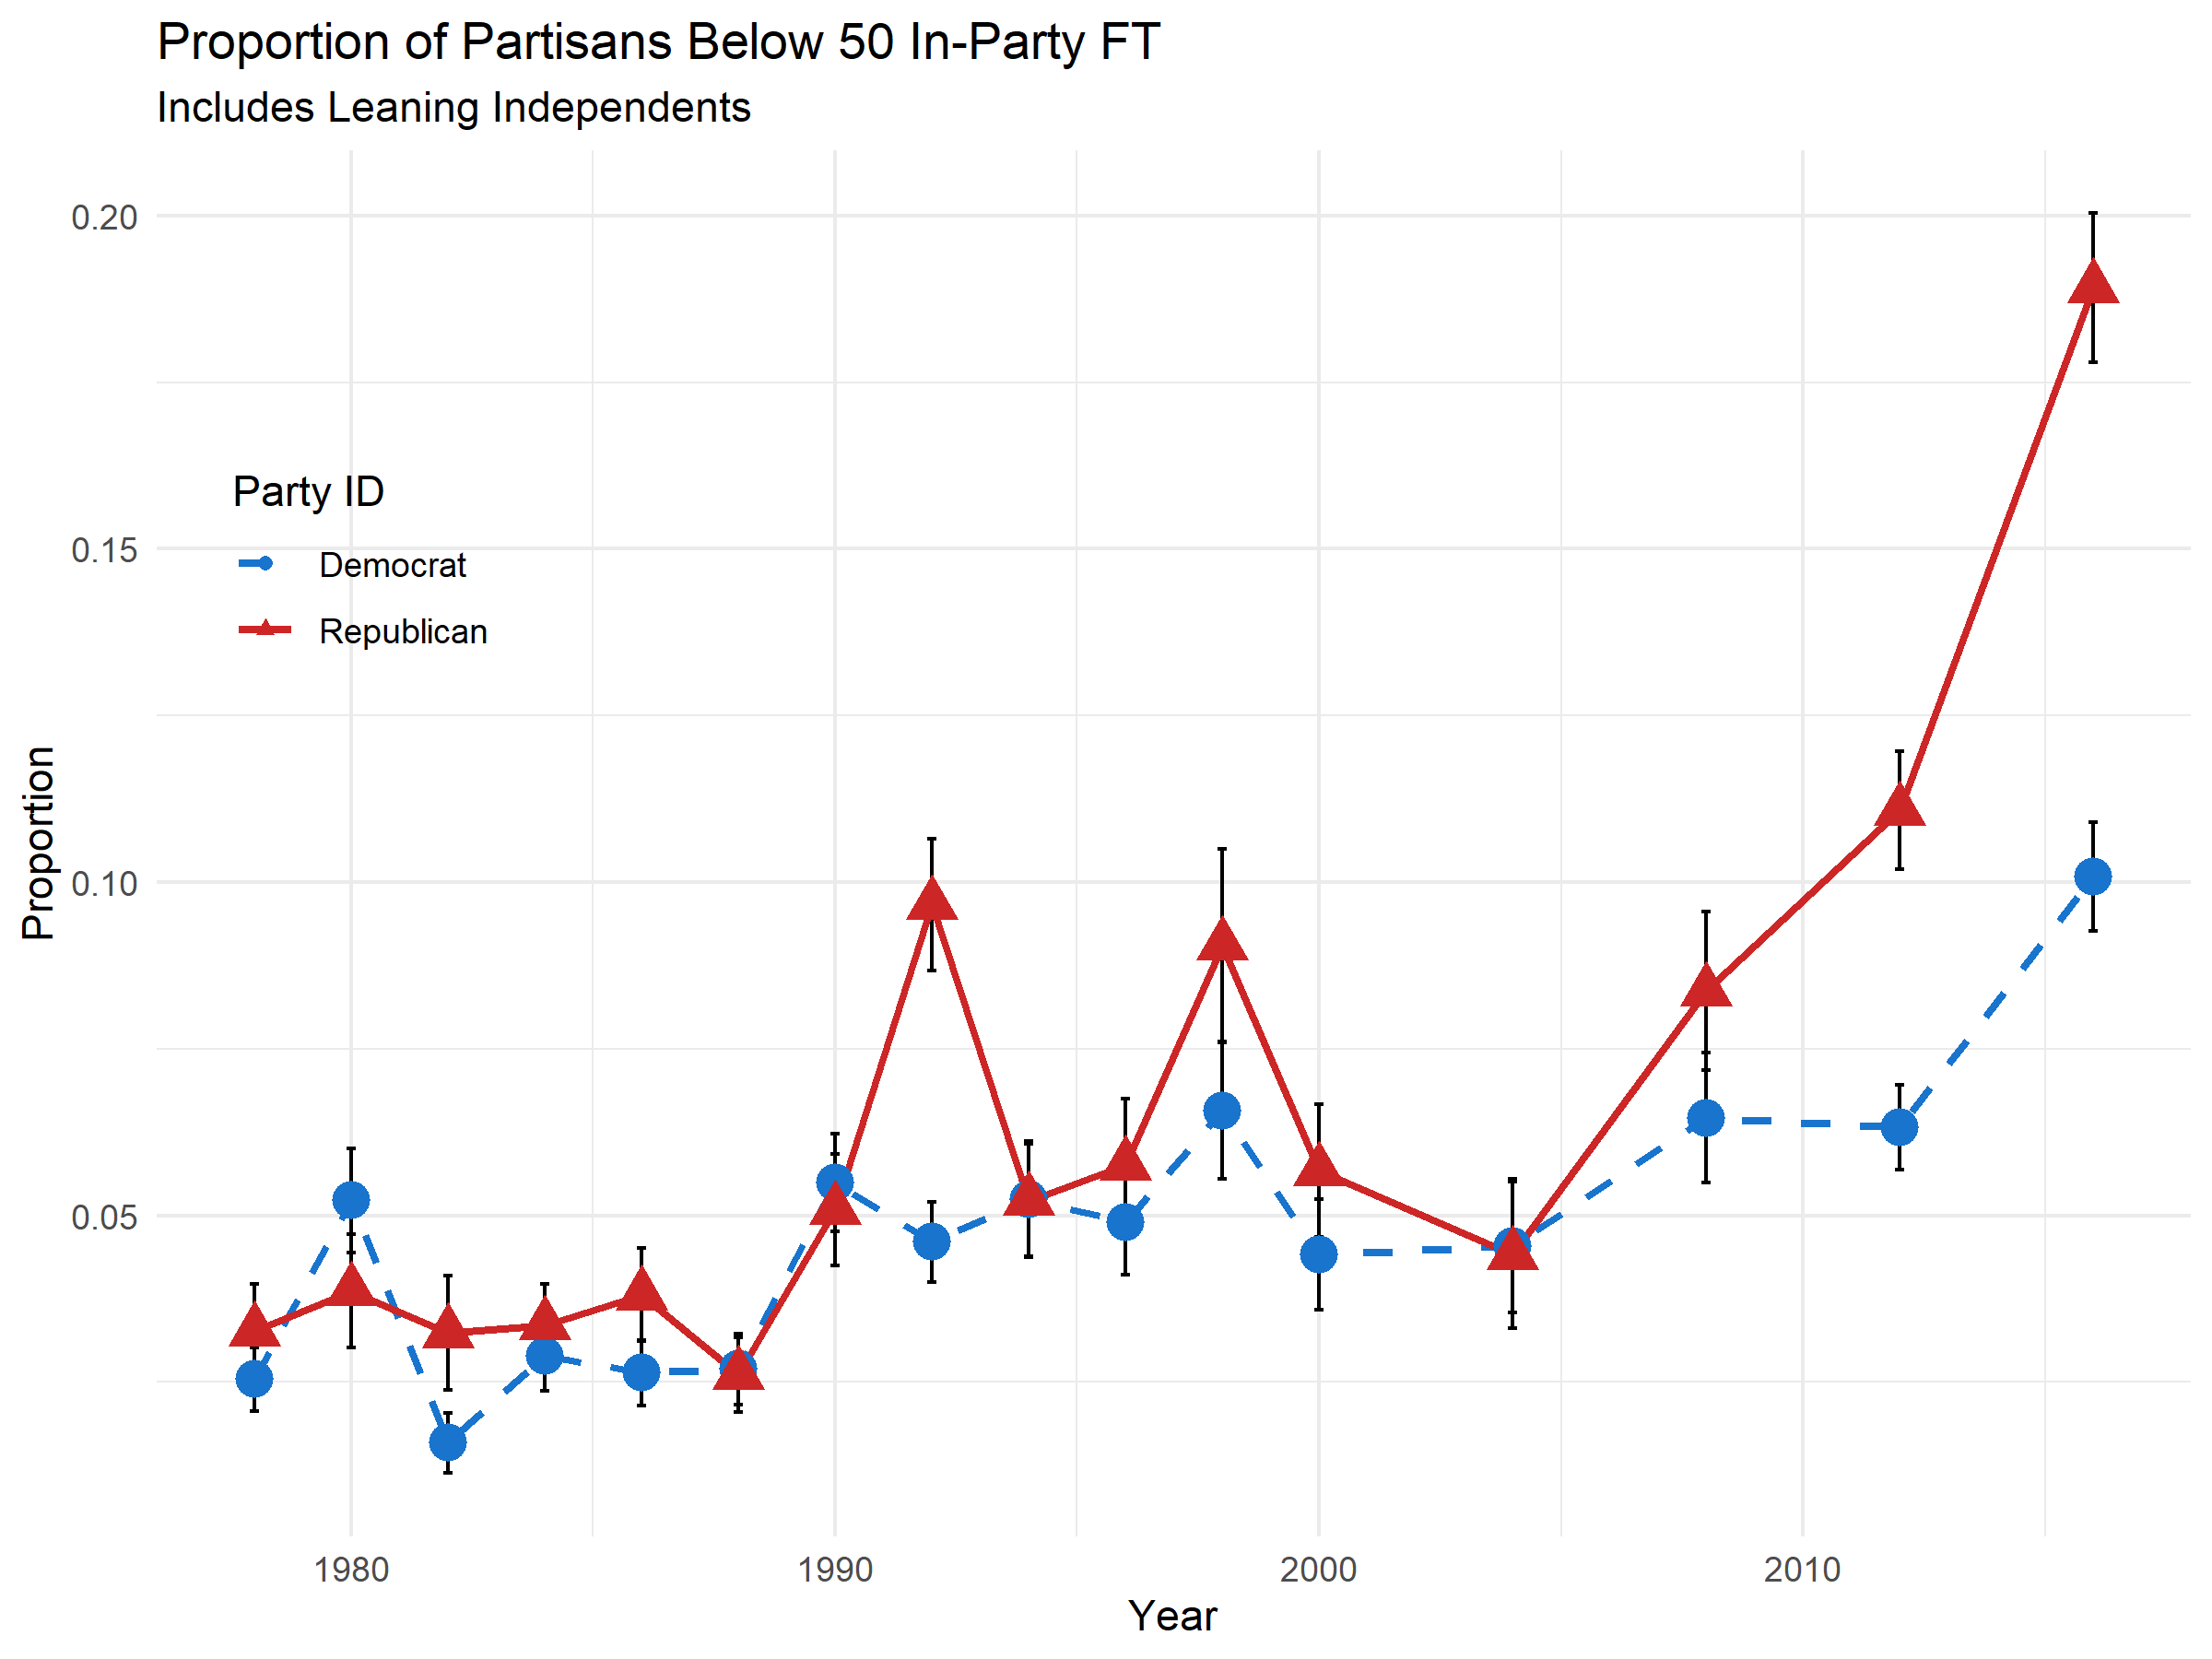
\includegraphics[width=.7\textwidth]{cdf-below-50-ns.png}
\caption{\label{fig:cdf-below-50} \textit{\textbf{The proportion of partisans who whose in-party FT falls below 50.} %Republicans and Democrats increasingly report feeling colder than the median.
}}
\end{wrapfigure}

The increasing frequency of cold in-party affect is shown in Figure \ref{fig:cdf-below-50}. In 2004, less than 5\% of Republicans and Democrats were cold toward their party, in 2016 that number increased to 10\% of Democrats and almost 20\% of Republicans. This trend is robust across all strengths of partisan identification and regardless of the score we deem to indicate coldness. Additional figures will made available in the appendix.



Finally, Figure \ref{fig:ridge} displays changes in the distribution of in-party FTs over time. From 2004--2016, the left tail has grown noticeably longer and more dense. While the majority of partisans remain warmer than 50, these figures are striking.

\begin{wrapfigure}{R}{.6\textwidth}
\centering
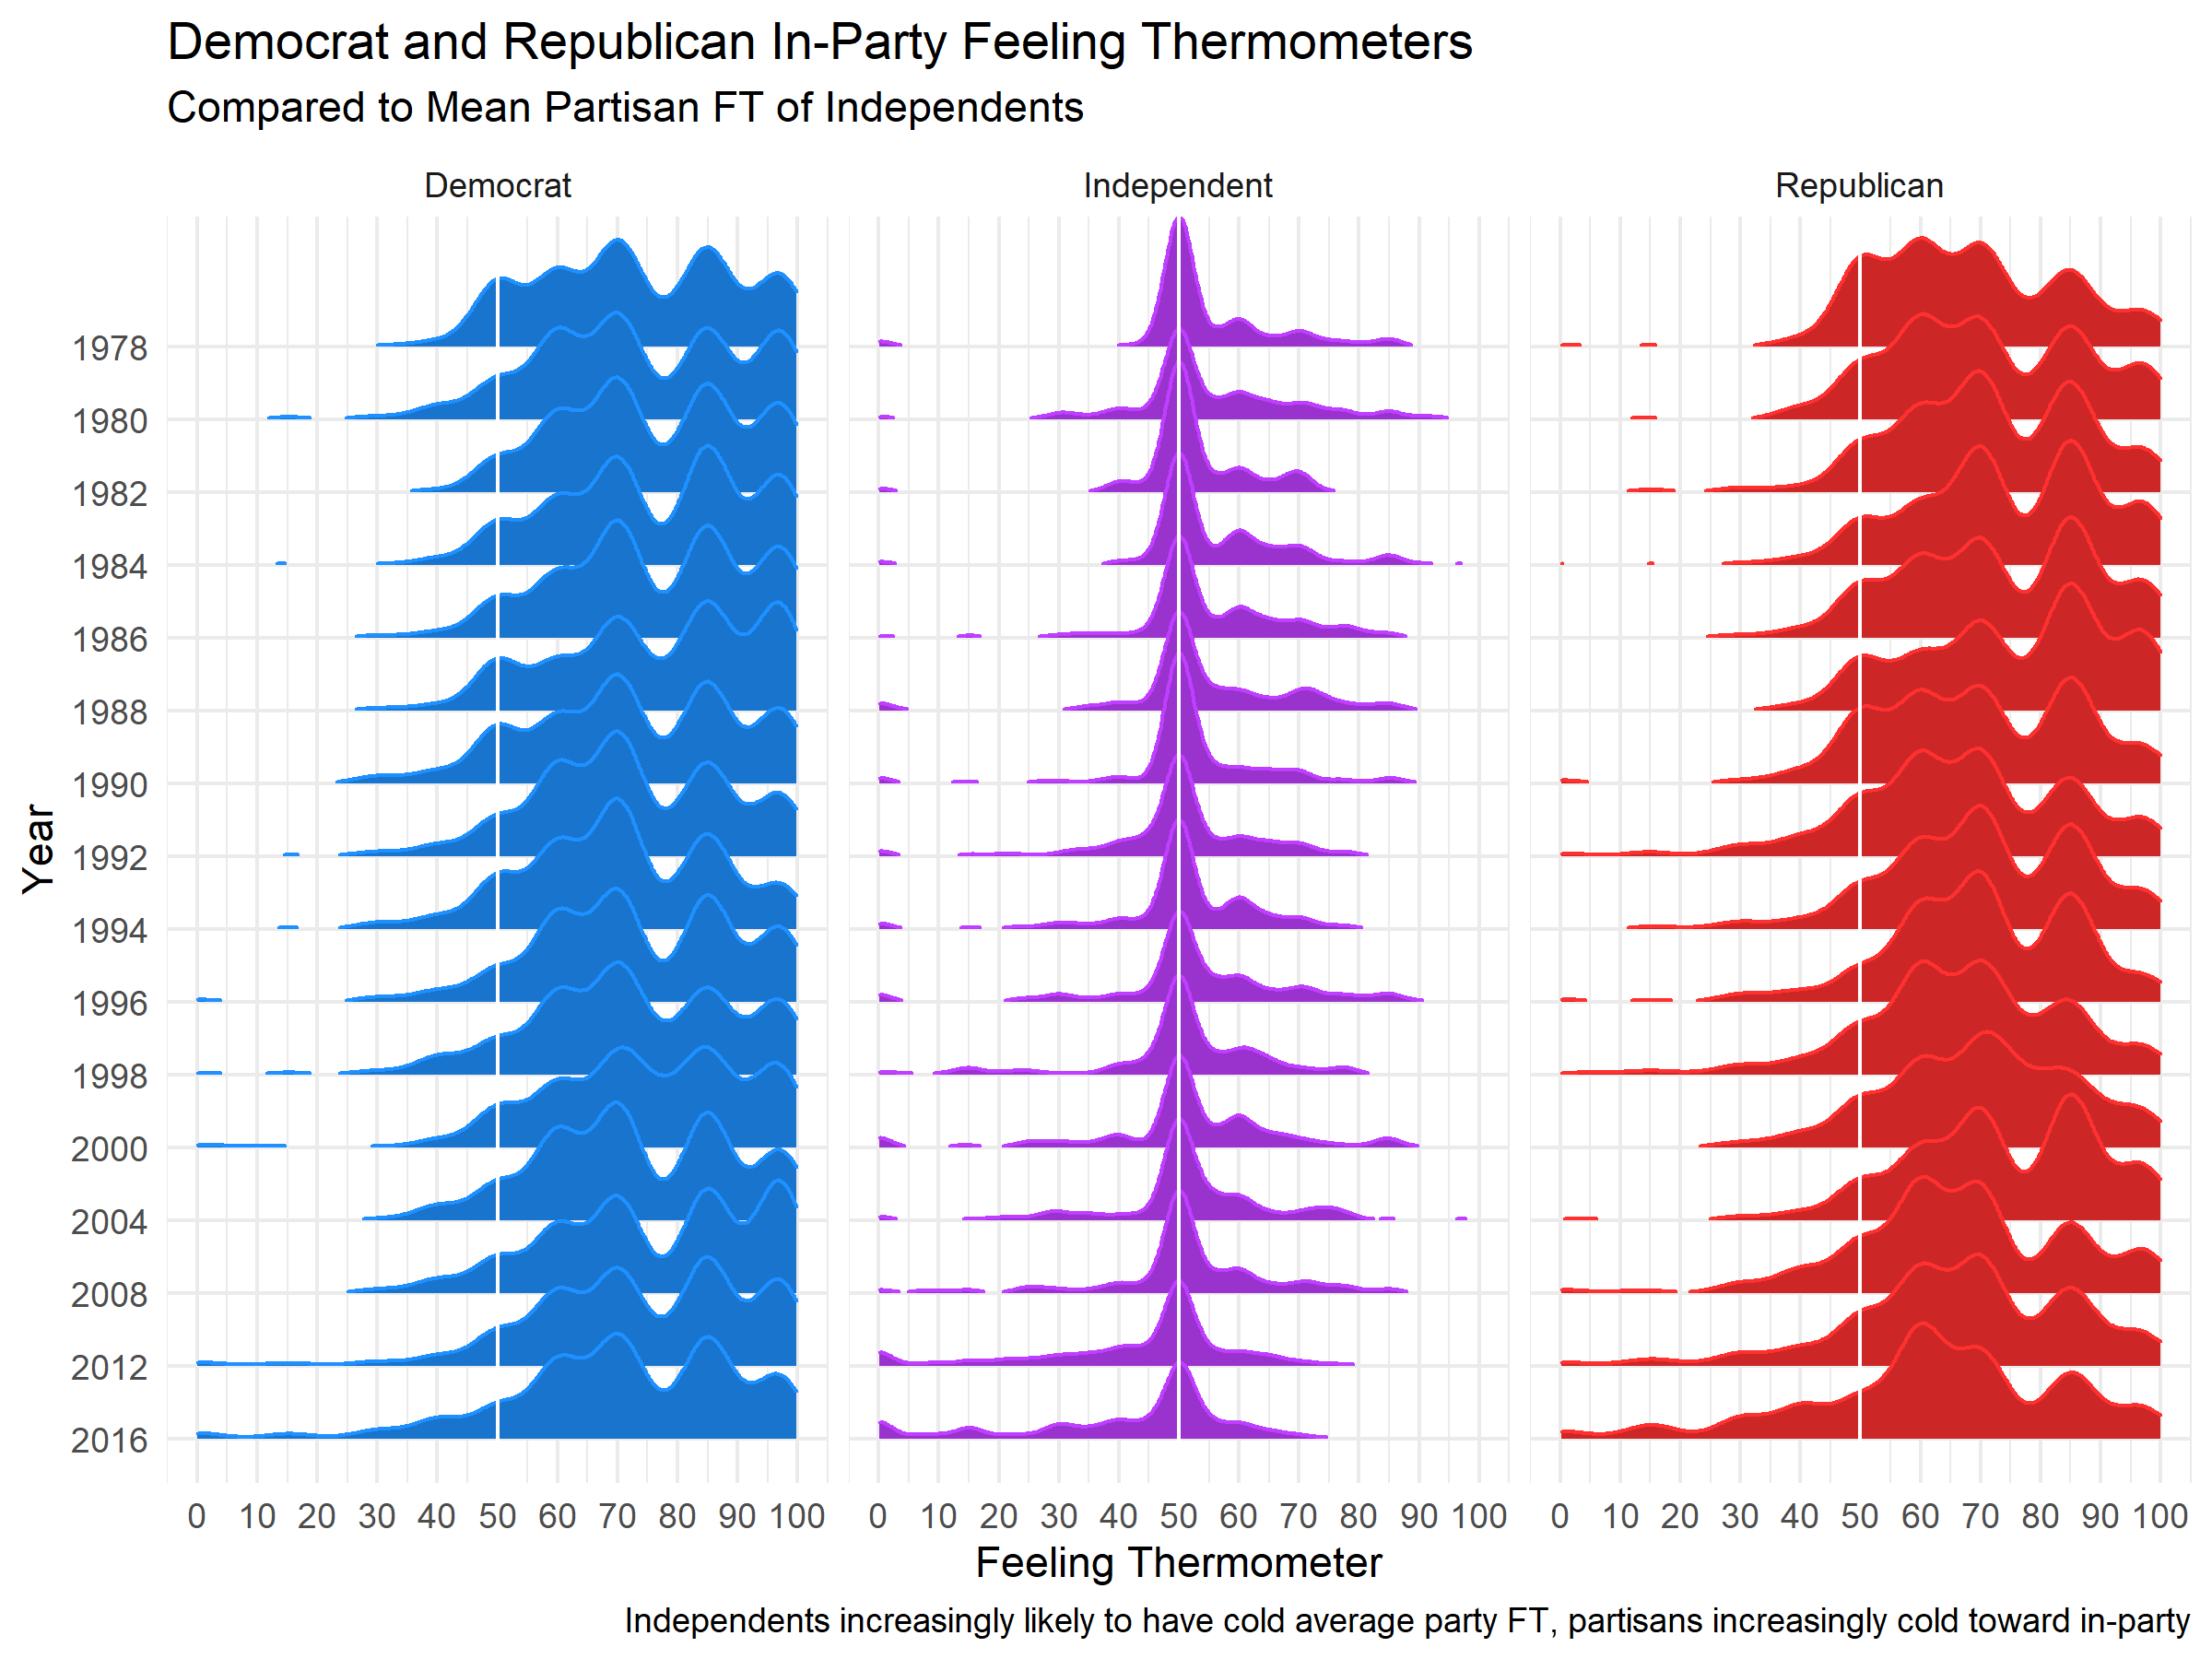
\includegraphics[width=.6\textwidth]{cdf-ridge-ns.png}
\caption{\label{fig:ridge} \textit{\textbf{Ridgeline plot of partisan feeling thermometers.} Partisans' in-party/independents average FT.}}
\end{wrapfigure}


\subsection{Dissatisfaction}

The findings presented here support the view of \cite{klar2018affective}, that the pattern of  affective partisan polarization identified in recent years (e.g. \citet{iyengar2012affect}), is better characterized as increasing frustration with political parties in general---not simple polarization. It is true that antipathy towards the outparty has increased since the 1970s, but so to has the proportion of those who are lukewarm or cold toward their own party.

This raises troubling normative concerns regarding citizens' faith in democracy. By the ANES's measure, the proportion of people ``Somewhat" or ``Very" dissatisfied with democracy has increased from about 18\% in 2004 (the first year the question was asked), to 34\% in 2012 and 2016.

\begin{wrapfigure}{R}{.7\textwidth}
\centering

\includegraphics[width=.7\textwidth]{cdf-ridge-all-dis.png}
\caption{\label{fig:ridge-dis} \textit{\textbf{Ridgeline plot of mean partisan feeling thermometers by reported satisfaction in democracy.} %Partisans' in-party/independents average FT. Plots show the distributions of mean partisan feeling thermometers---$(FT_D + FT_R)/2$---of those satisfied and dissatisfied with Democracy. Unsurprisingly, those dissatisfied are more likely to have a cold average FT
}}
\end{wrapfigure}

Figure \ref{fig:ridge-dis} shows all respondents' mean partisan feeling thermometer (the average of their Democrat and Republican thermometers), stratified by whether the respondent is satisfied or dissatisfied with Democracy. Unsurprisingly, the leftward tails are largest among discontents, but all three groups (satisfied, dissatisfied, and those who weren't sure or declined to answer) have become increasingly likely to be, an average, cold towards the parties.

\subsection{Primaries}
Setting aside issues of causal identification, clearly increasing dissatisfaction with democracy does not fully explain  the increase in those who are cold toward their (or both) parties\footnote{Nor does cold partisan affect explain all increasing dissatisfaction.}. I turn now to an examination of the relationship between primary vote choice and in-party affect. I argue that the increase in cold partisan affect can be explained in part by ``sore losers" in primary elections---as primaries become more salient, so to do the factions represented by supporters of particular candidates. In short, primary elections provide another layer of group-based political identity below the party, forcing partisans to see not just the out-party as adversarial, but members of their own party as well.

\begin{wrapfigure}{R}{.75\textwidth}
\centering
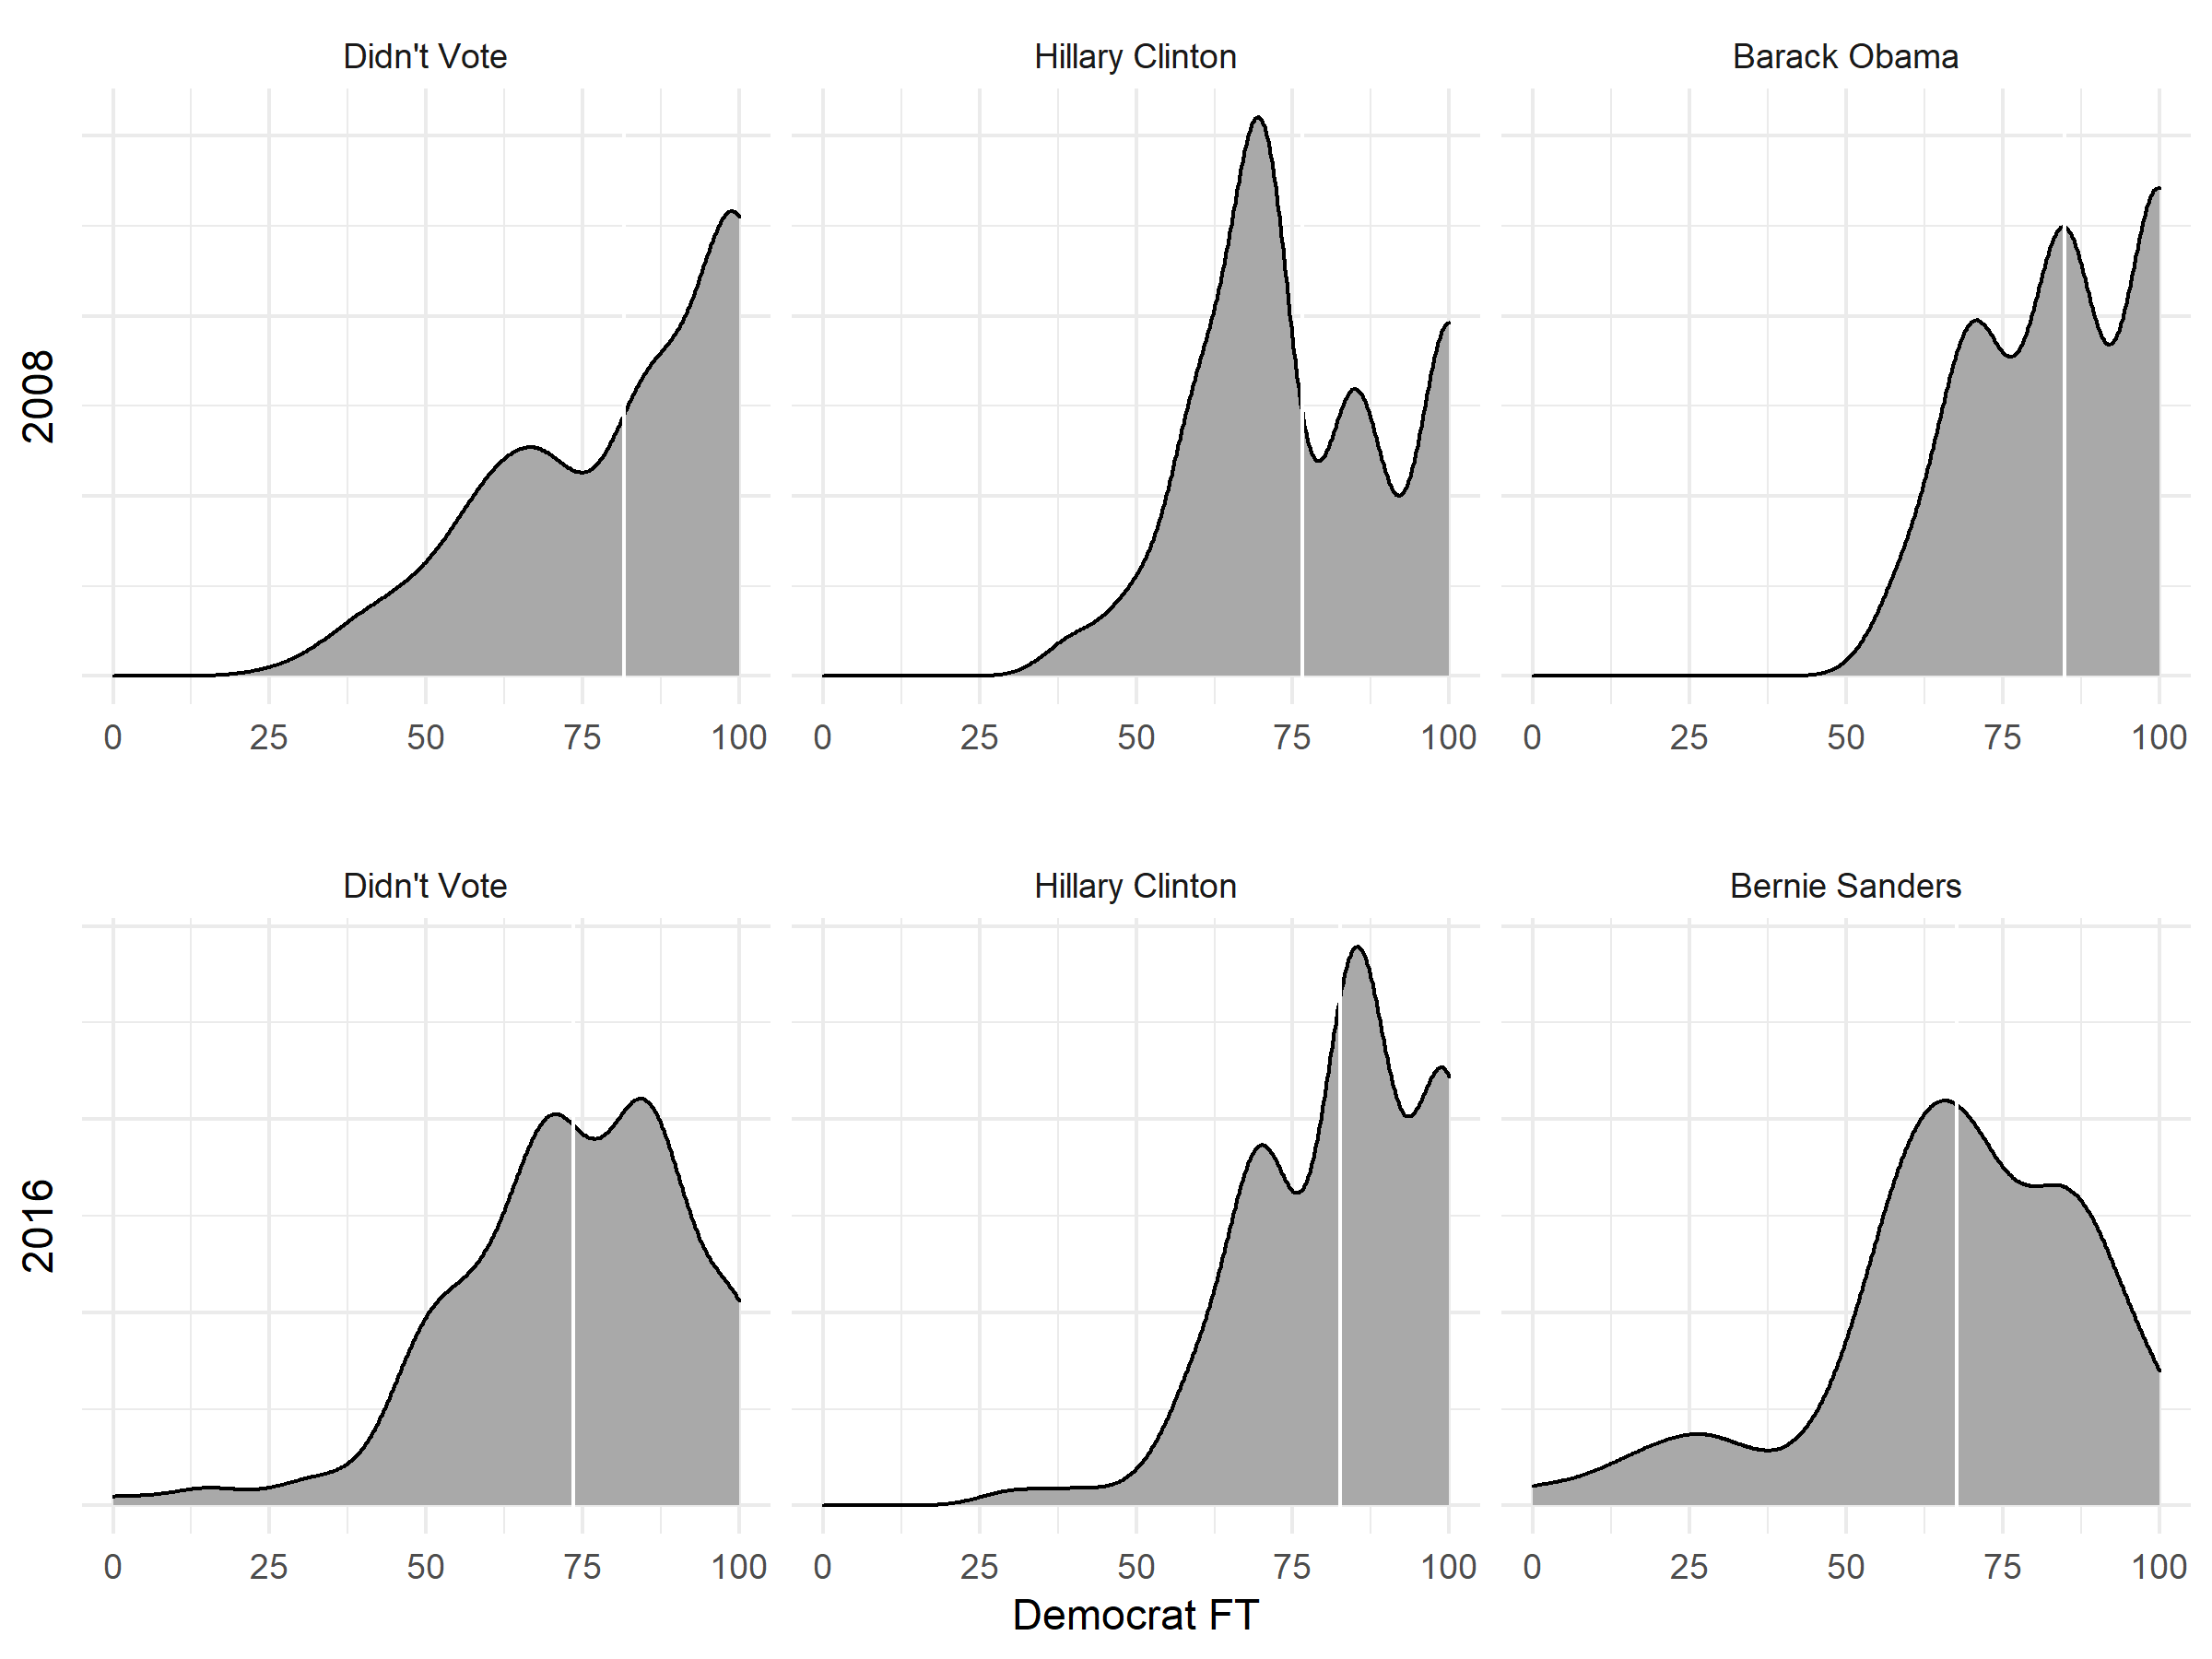
\includegraphics[width=.7\textwidth]{primary-dem.png}
\caption{\label{fig:primary-dem} \textit{\textbf{Density plots of in-party feeling thermometers by year and primary candidate preference.}}}
\end{wrapfigure}
 Primary elections are substantively significant events, allowing partisans a voice in the presentation and direction of their party. In a political environment in which the presidential nominee becomes the de facto leader of the party, the primary process affords non-elite voters a voice in the ideological, political, and stylistic future of the party. The political products offered by primary candidates may reflect (or drive) extant divisions in the party. \cite{wronski2018tale} and \cite{bankert2020authoritarian} find that those scoring highly on measures authoritarian personality traits use their primary vote to ``protect" their party from factions they see as threatening group cohesion. Just as voters do not toss a coin to decide their general election vote, they do not randomly select their choice in the primary; these choices are likely to be meaningful. 

Figure \ref{fig:primary-dem} shows density plots of Democrats' in-party feeling thermometers in 2008 and 2016 in each year, in both years, those who supported a losing candidate were more more likely to be cold to their party than even non-voters. One might suspect a reverse causal relationship---that the 2016 data are a product of Sanders supporters' predisposition against their party. While some Sanders supporters were no doubt motivated by an \textit{a priori} disdain for the establishment, note the large number of lukewarm Clinton Democrats relative to both Obama supporters and nonvoters. It would be difficult to imagine a more establishment Democrat than Hillary Clinton running against Obama---then a young senator promising to upset the status-quo.

On the Republican side, the Trump campaign postured itself as openly hostile to the Republican party, perhaps even to a greater degree than did the Sanders campaign against the Democrats. Despite this, Trump supporters were the warmest group of Republican primary voters\footnote{[Figs will be updated to include reps]}---bad news for our \textit{a priori} disdain hypothesis---and good news for the sore loser hypothesis.

\begin{figure}
\centering

\includegraphics[width=1\textwidth]{partisan-loess-all.png}
\caption{\label{fig:loess} \textit{\textbf{LOESS model estimating probability of self-identifying as a strong partisan}}}
\end{figure}

\subsubsection{Panel Data}

Based on cross-sectional data alone it is unclear whether vote choice or a cold affect is prior to the other. Using panel data from the 2000 and 2008 presidential elections

%The main lesson of this study to scholars of political polarization should be the importance of clearly conceptualizing what is substantively important about polarization, and understanding the methodological trade-offs that occur when too much is built in to our dependent-variable models of polarization. The tacit (or explicit) assumption that in-party feelings are necessarily high when out-party feelings are low should be put to rest.

%Given that partisans feelings towards their own party are not necessarily predictive of their feeling toward the opposing party, political scientists should carefully consider what substantive questions they are interested in asking when justifying a choice of dependent variable, recognizing that choice can limit the number of questions which can be asked, and obscure potential insights.

%If scholars' interest in affective polarization is truly in the distance between partisans' assessments of themselves and their opponents, a measure like net partisan affective is appropriate. If, however, the researcher's interest is in the absolute political hostility or animus \textit{implied} by that distance, they should simply use partisan's direct feelings towards their enemies. There is no reason for those in the latter camp to run the risk of overcomplicating an analysis or confounding an interesting result by including in their measure a variable unrelated to their interests.
%\subsection{Research Design Concerns and Limitations}
%\begin{figure}[H]
%\center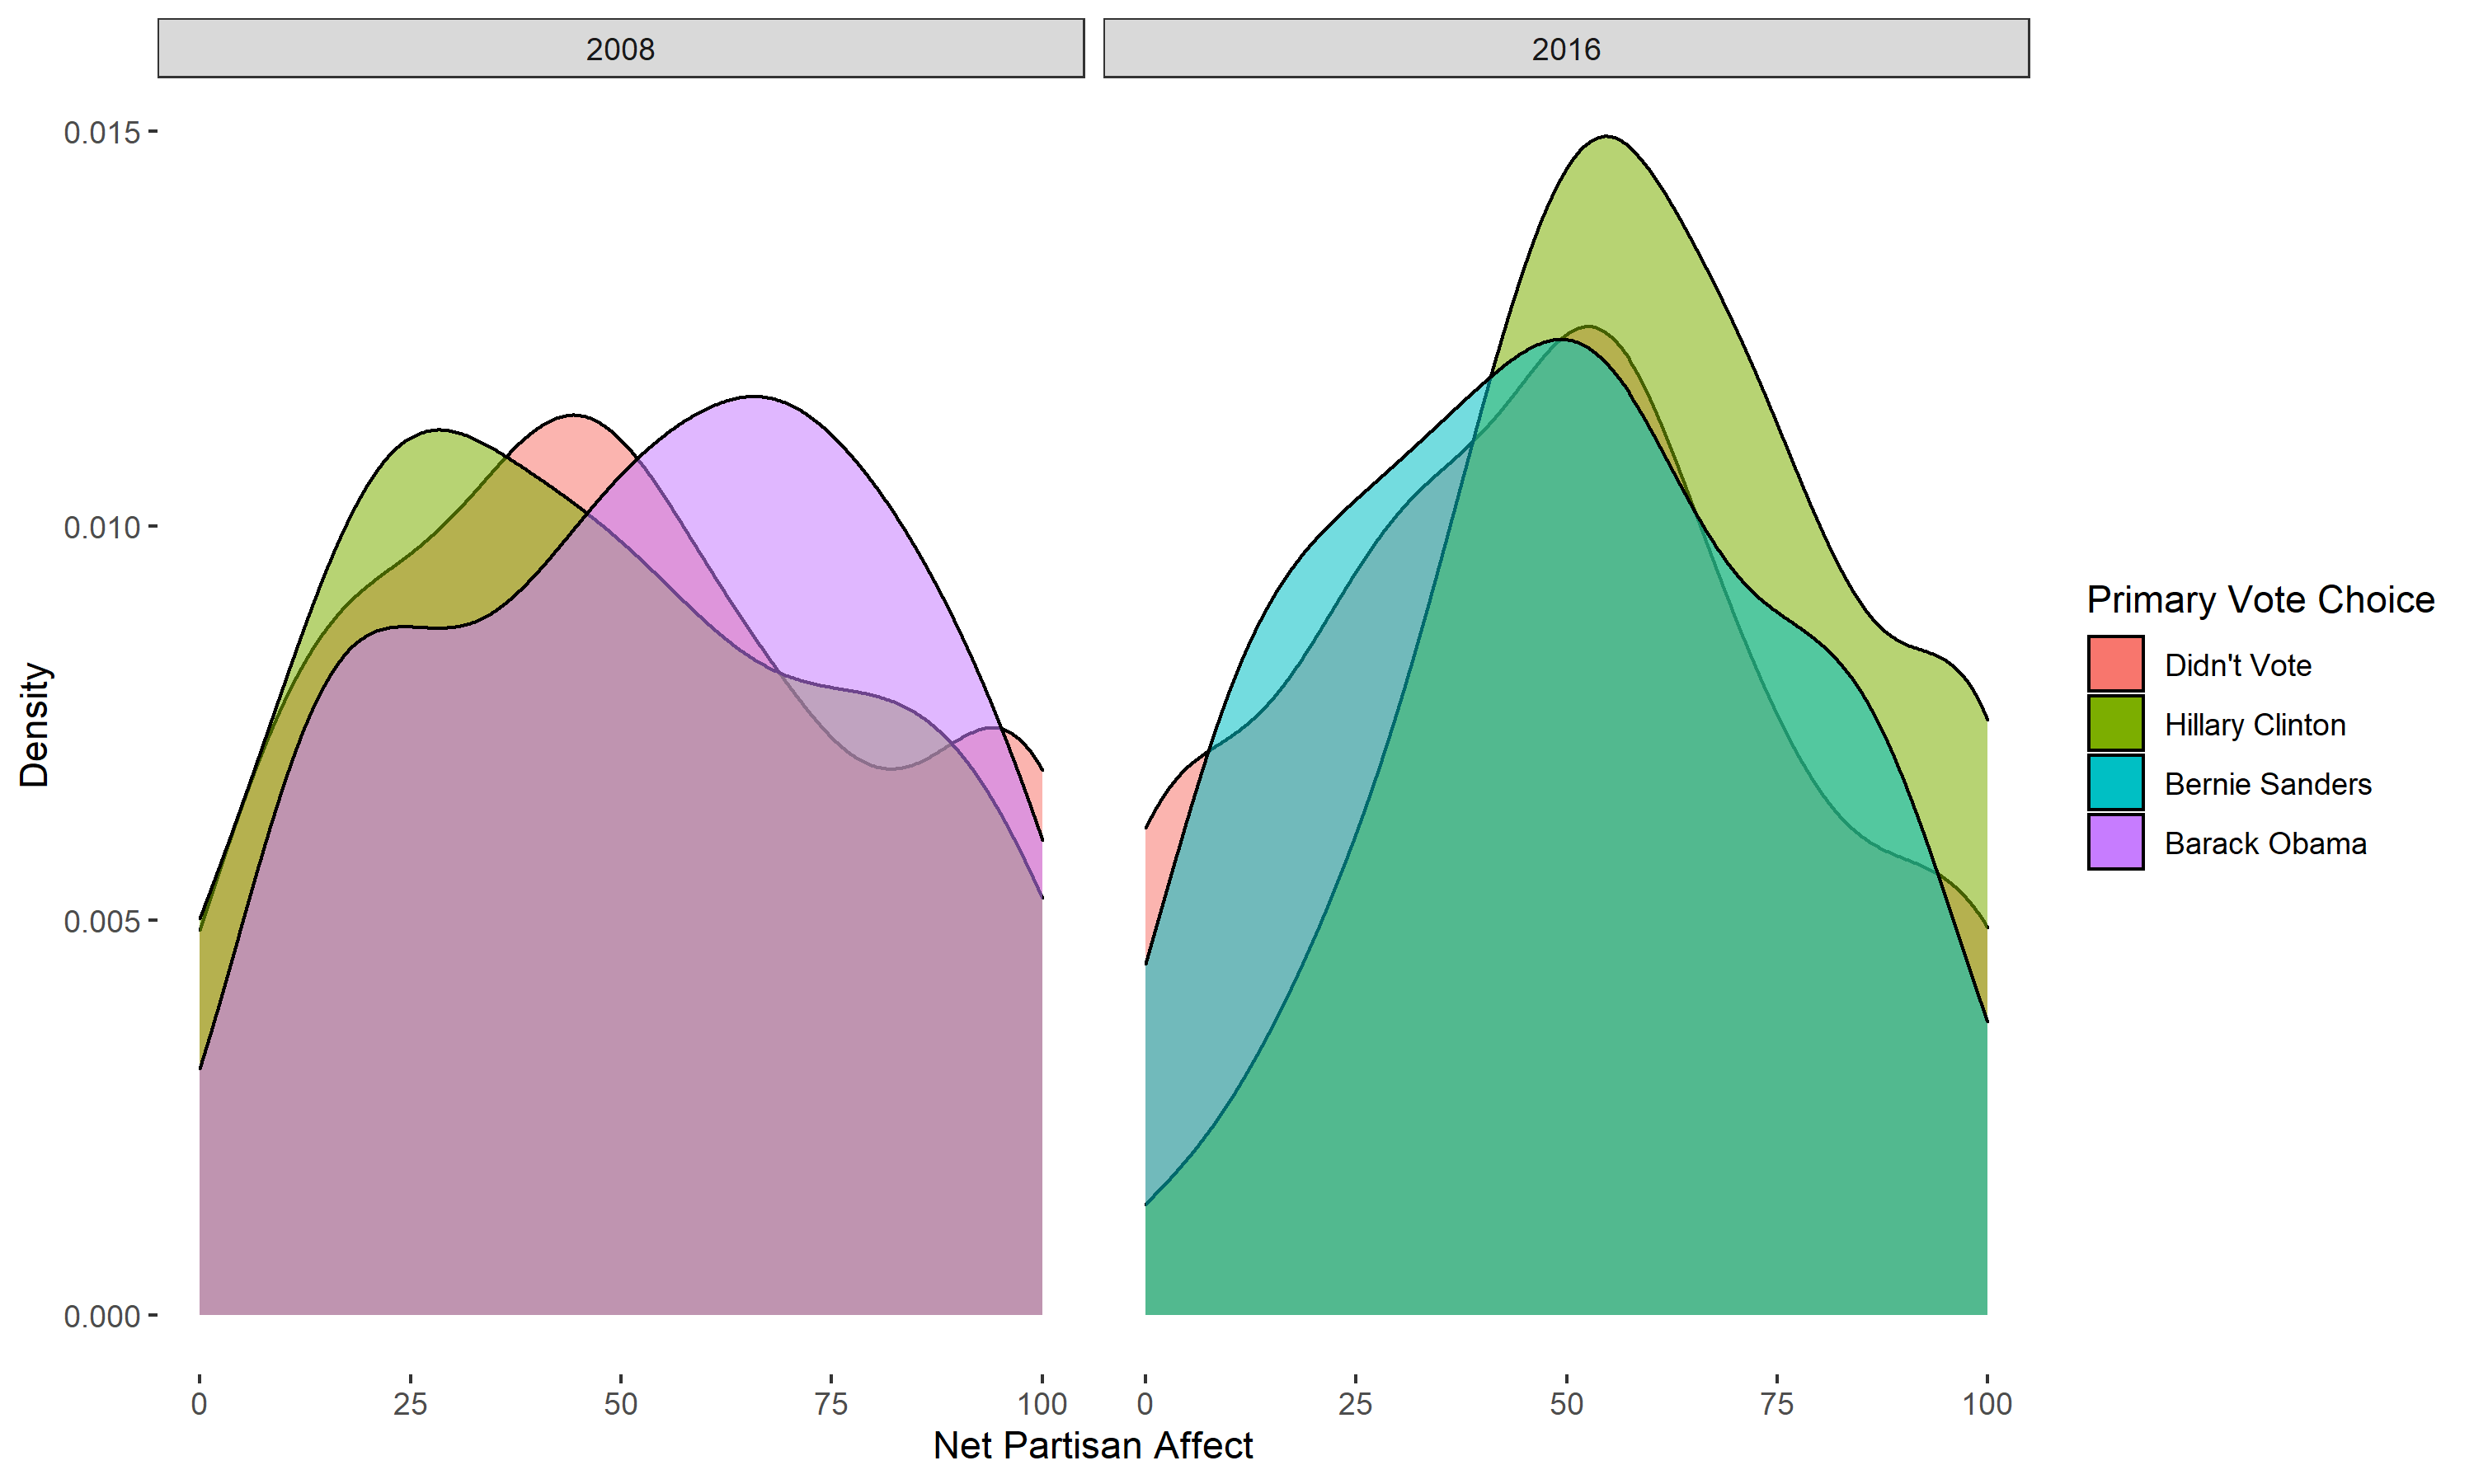
\includegraphics[width=6in]{therm-hist-2016.png}
%\caption{\label{fig:dens}\textit{Density plots of net partisan affect by vote in primary elections}.}
%\end{figure}

%These data are obviously quite limited, looking at members of one party across two years, but they should motivate additional research.


%compare decrease in NPA of losers to average NPA decrease of losers.



\thispagestyle{empty}
\clearpage
\setstretch{1}
\bibliography{references}
%\section{Appendix}



%\subsection{ISL's Model Extended to 2016}



%
%\section{Intra-Party Affect \& Primaries}
%
%In this section, I motivate an extension to \citet{iyengar2012affect}, drawing on partisanship and feeling thermometer data from the ANES-CDF to present time-series trends in Democrats' affect toward their party and the Republican Party. I show, consistent with extant literature, mean out-party feeling thermometers have been decreasing since the late \nth{20} Century. However, the mean feeling thermometers of the parties writ-large do not provide a sufficiently nuanced view of citizens' affect.
%
%\subsection{Internal Division}
%Extant scholarship has, in large part, treated the major parties as affectively monolithic; party ID is assumed the least common denominator of political identity. It is also commonly assumed that warmth toward the in-party is (and has been) high across all partisans \citep{iyengar2012affect}. 
%
%
% While affective polarization between partisans \textit{is} very high at present, there is also reason to be suspicious of internal divisions \textit{within} each party. \cite{mason2018ideologues} finds that, in addition to partisan identity, citizens hold ideological identities. In other words, individuals see themselves not just as ``Democrats" and ``Republicans", but as ``liberals" and ``conservatives". These  ideological and partisan identities are related to one another, but suggest that political identities which cross cut partisanship are theoretically plausible.
%
%%\begin{figure}[H]
%%\center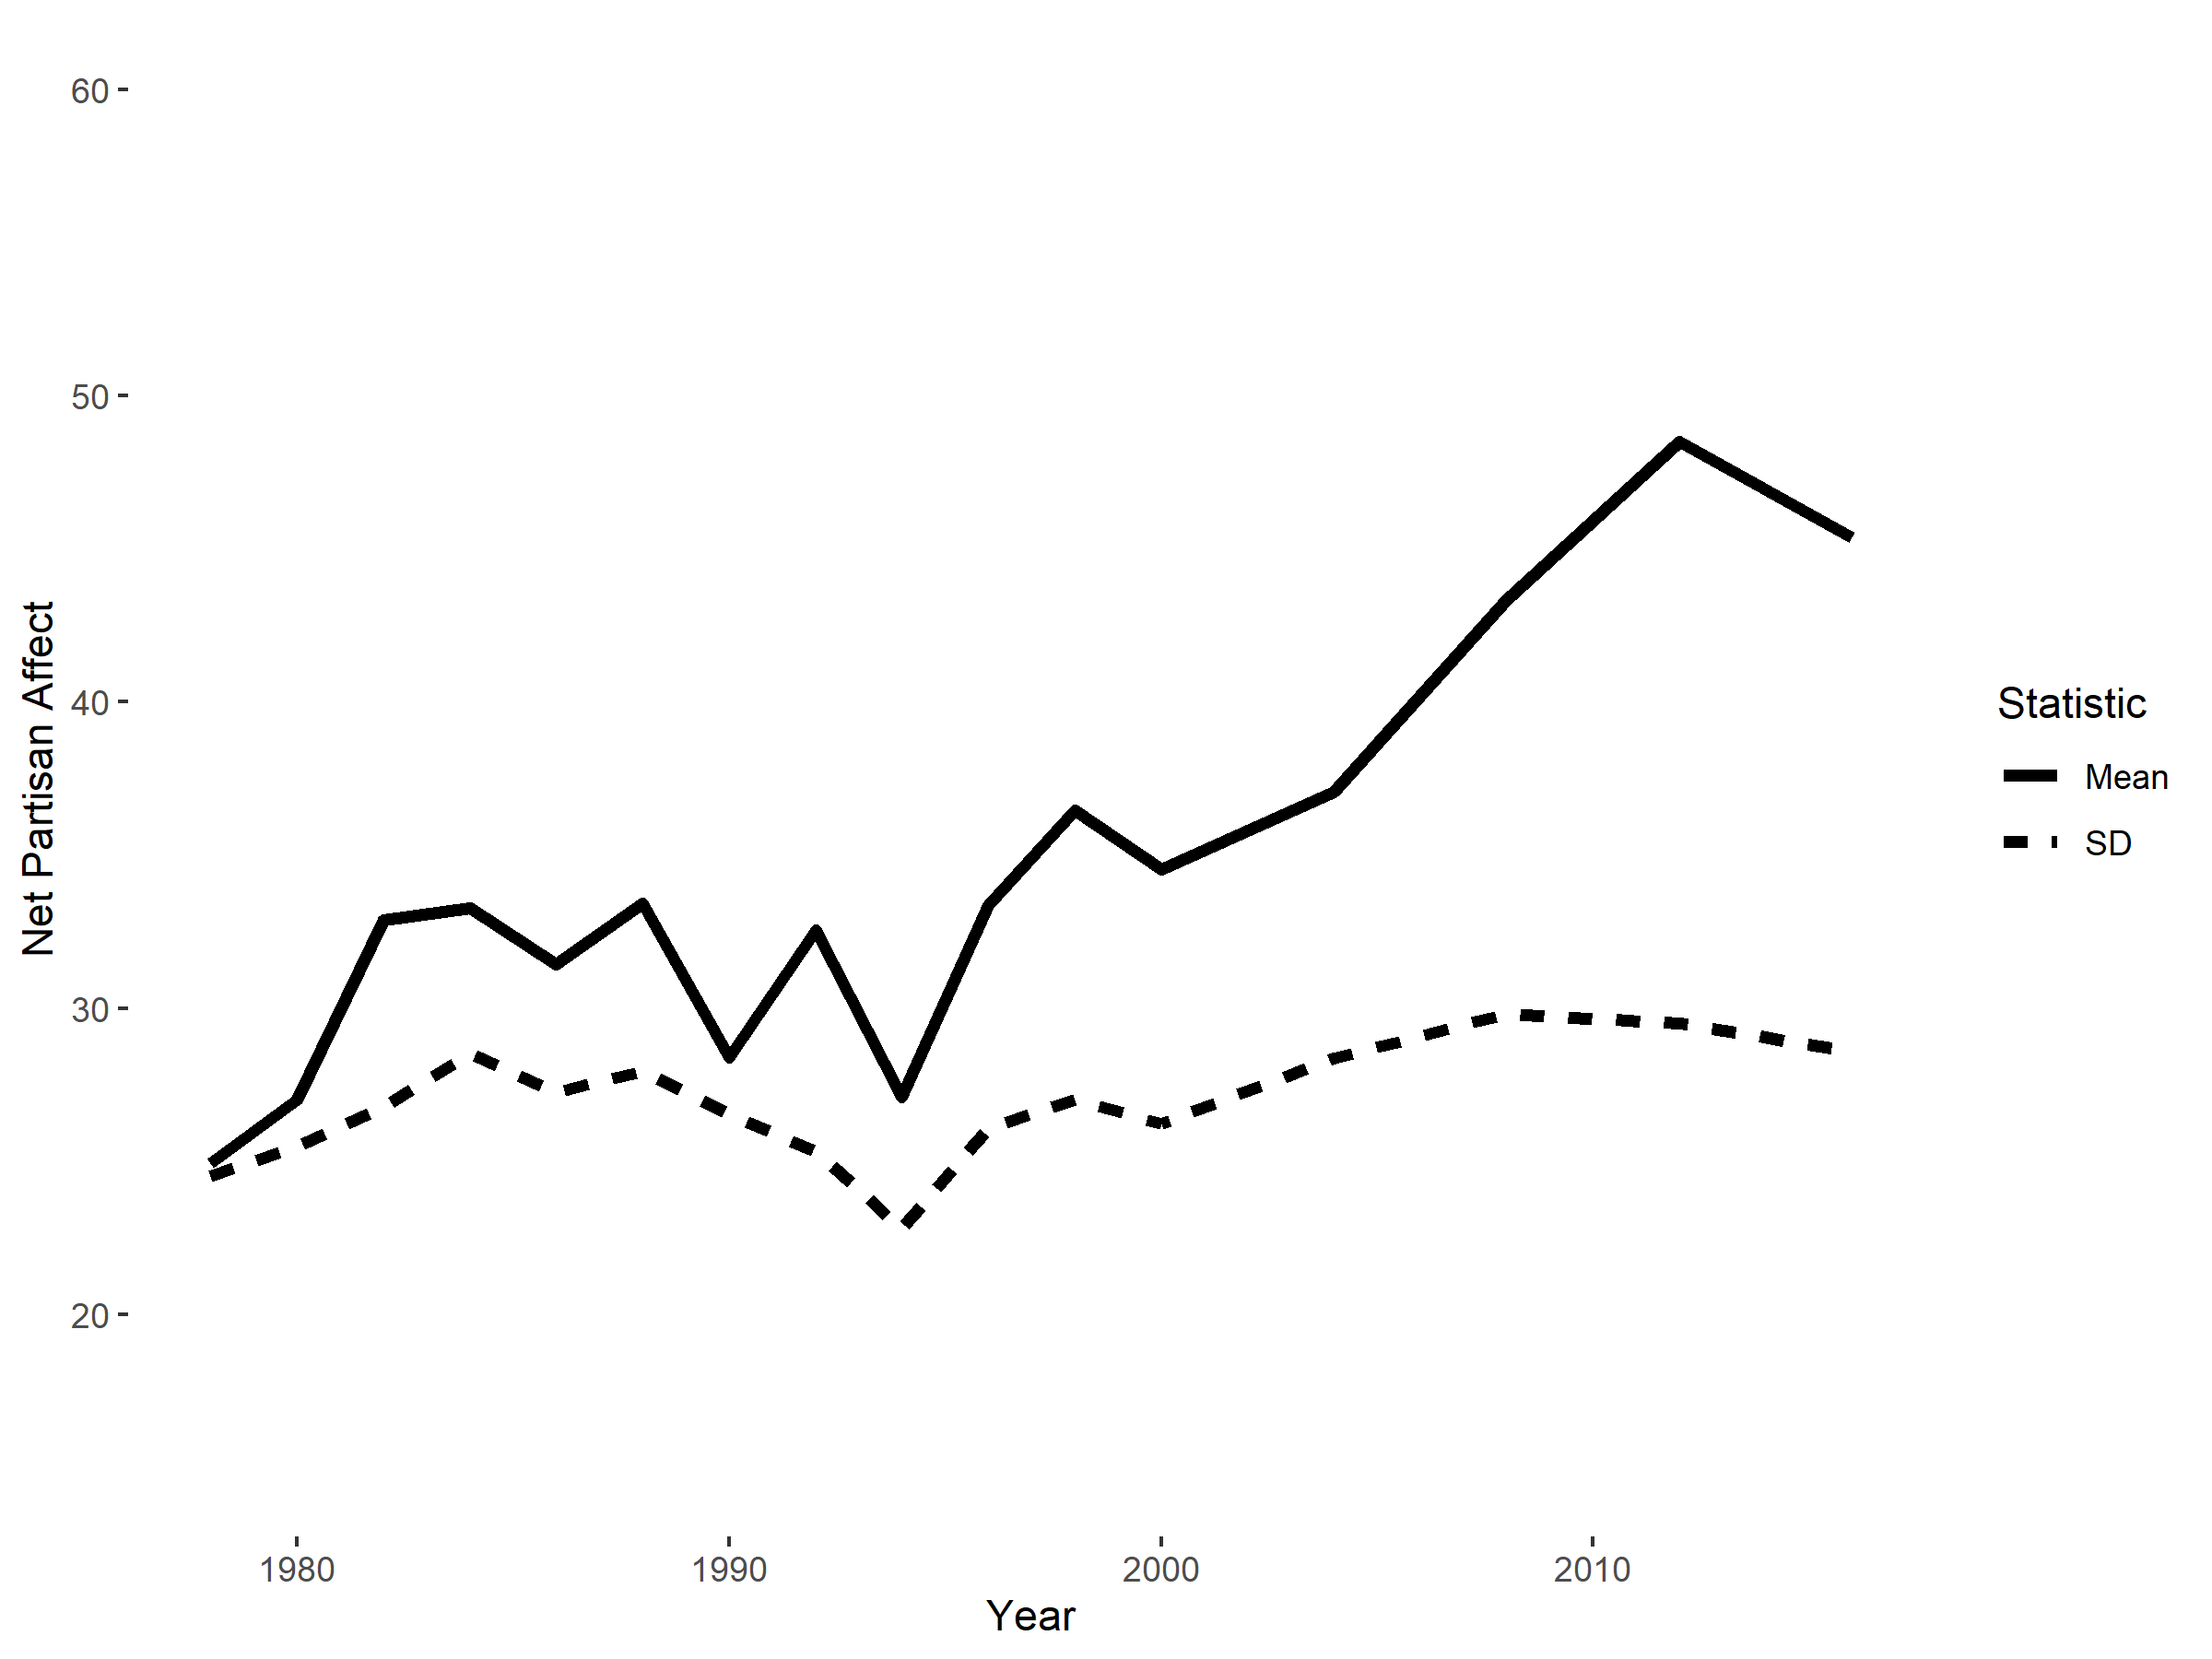
\includegraphics[width=6in]{cdf-npa.png}
%%\caption{\label{fig:cdf-npa} \textit{\textbf{Democrats Net Partisan Affect Since 1978.} NPA has increased, but so has the variance. Subtracting in-party FT from out-party FT obscures variation occurring in each measure.}}
%%\end{figure}
%\begin{figure}[H]
%\center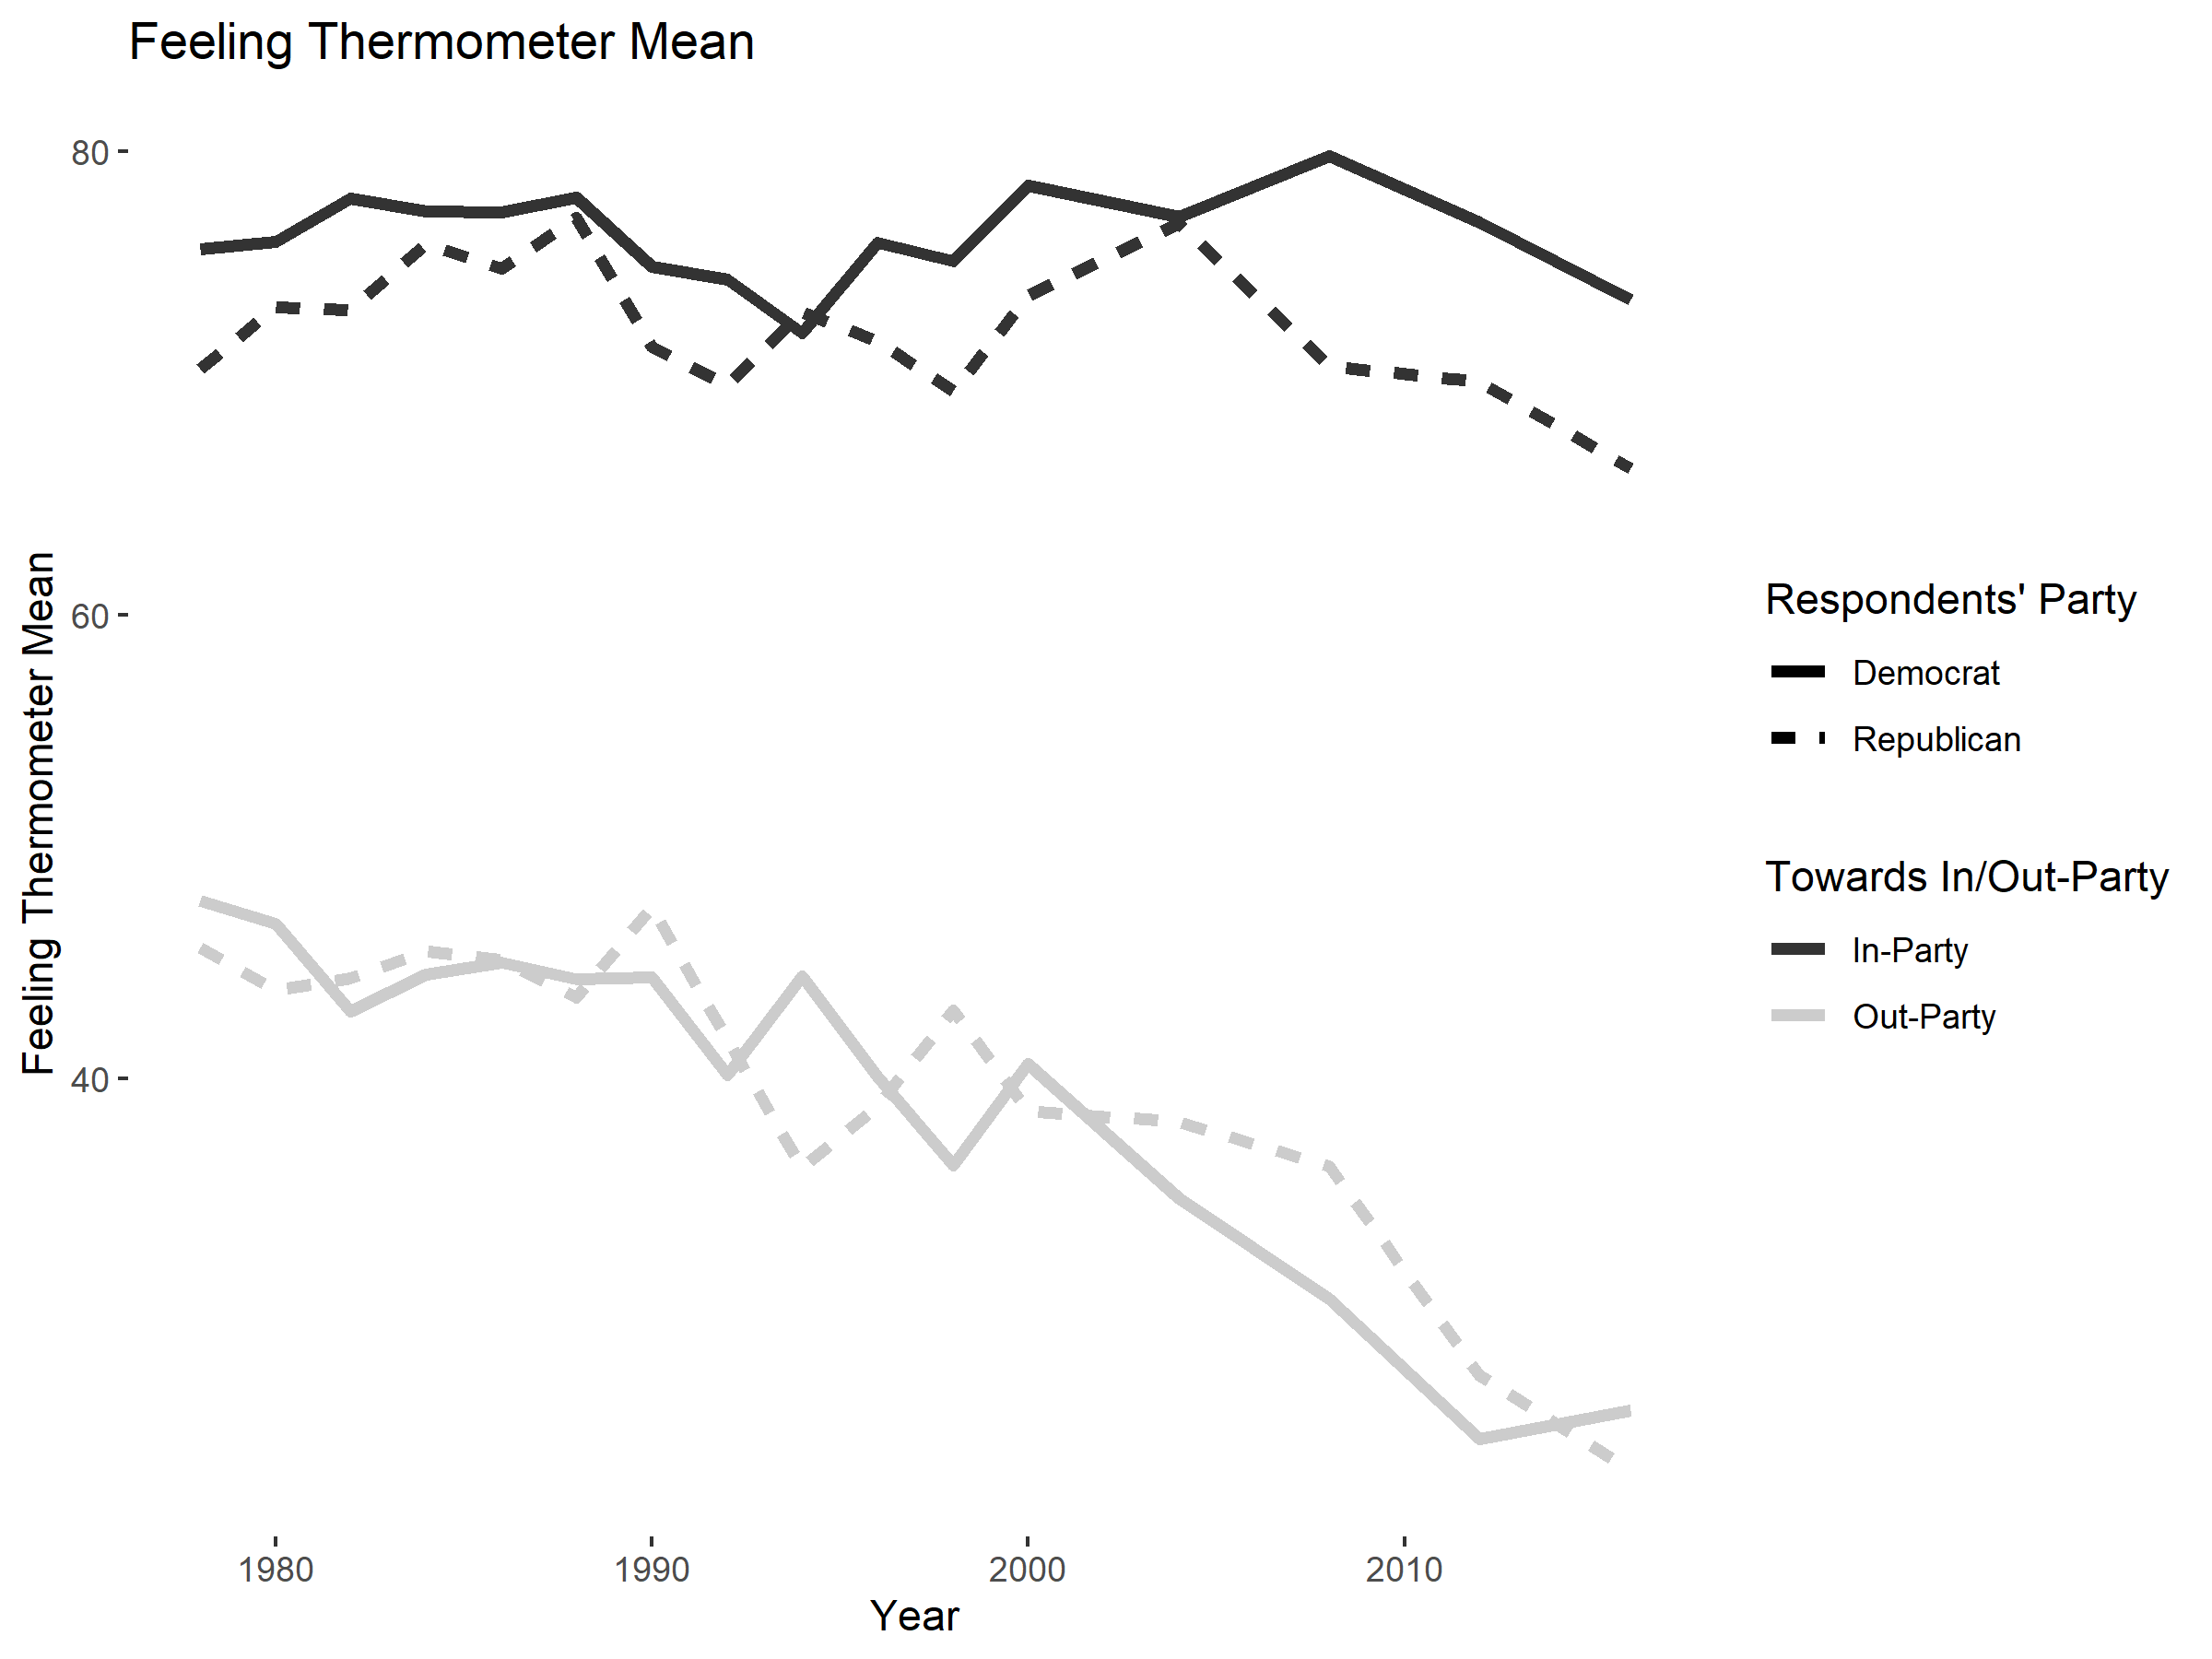
\includegraphics[width=5in]{cdf-avg.png}
%\caption{\label{fig:cdf-avg}\textit{\textbf{Yearly mean of partisans' in-party and out-party feeling thermometers, 1978--2016.} Consistent with the extant literature (e.g., \citet{iyengar2012affect}, Democrat and Republican in-party FTs are consistently high (with a slight decrease since the first decade of the 2000s).}}
%\end{figure}
%\noindent Figure \ref{fig:cdf-avg} shows the average in-party and out-party feeling thermometer for Republicans and Democrats from 1978-2016. We clearly see out-party feeling thermometers scores decline; while the in-party remains relatively constant. This is true of both parties.
%
%Unfortunately reliance on annual means as a description of partisan affect paints too simple a picture. The standard deviation of the feeling thermometers, presented in figure \ref{fig:cdf-sd}, shows that the stability of mean in-party affect observed in Figure \ref{fig:cdf-avg} belies an increase in the variation around that mean. This variation has increased in each iteration of the survey since 2004, both Republicans and Democrats have become less cohesive in their feelings toward their own party than at any other time period for which we have data. It should be noted that, historically, partisans are less cohesive in their feelings towards the out-party, though the variance in intra-party affect now seems to be on par with out-party feelings. %Both figures \ref{fig:cdf-sd} and \ref{fig:cdf-avg}are reproduced in the Appendix using data from Democrat leaning independents, to similar results.
%
%%%%%%%
%
%
%\begin{figure}[H]
%\center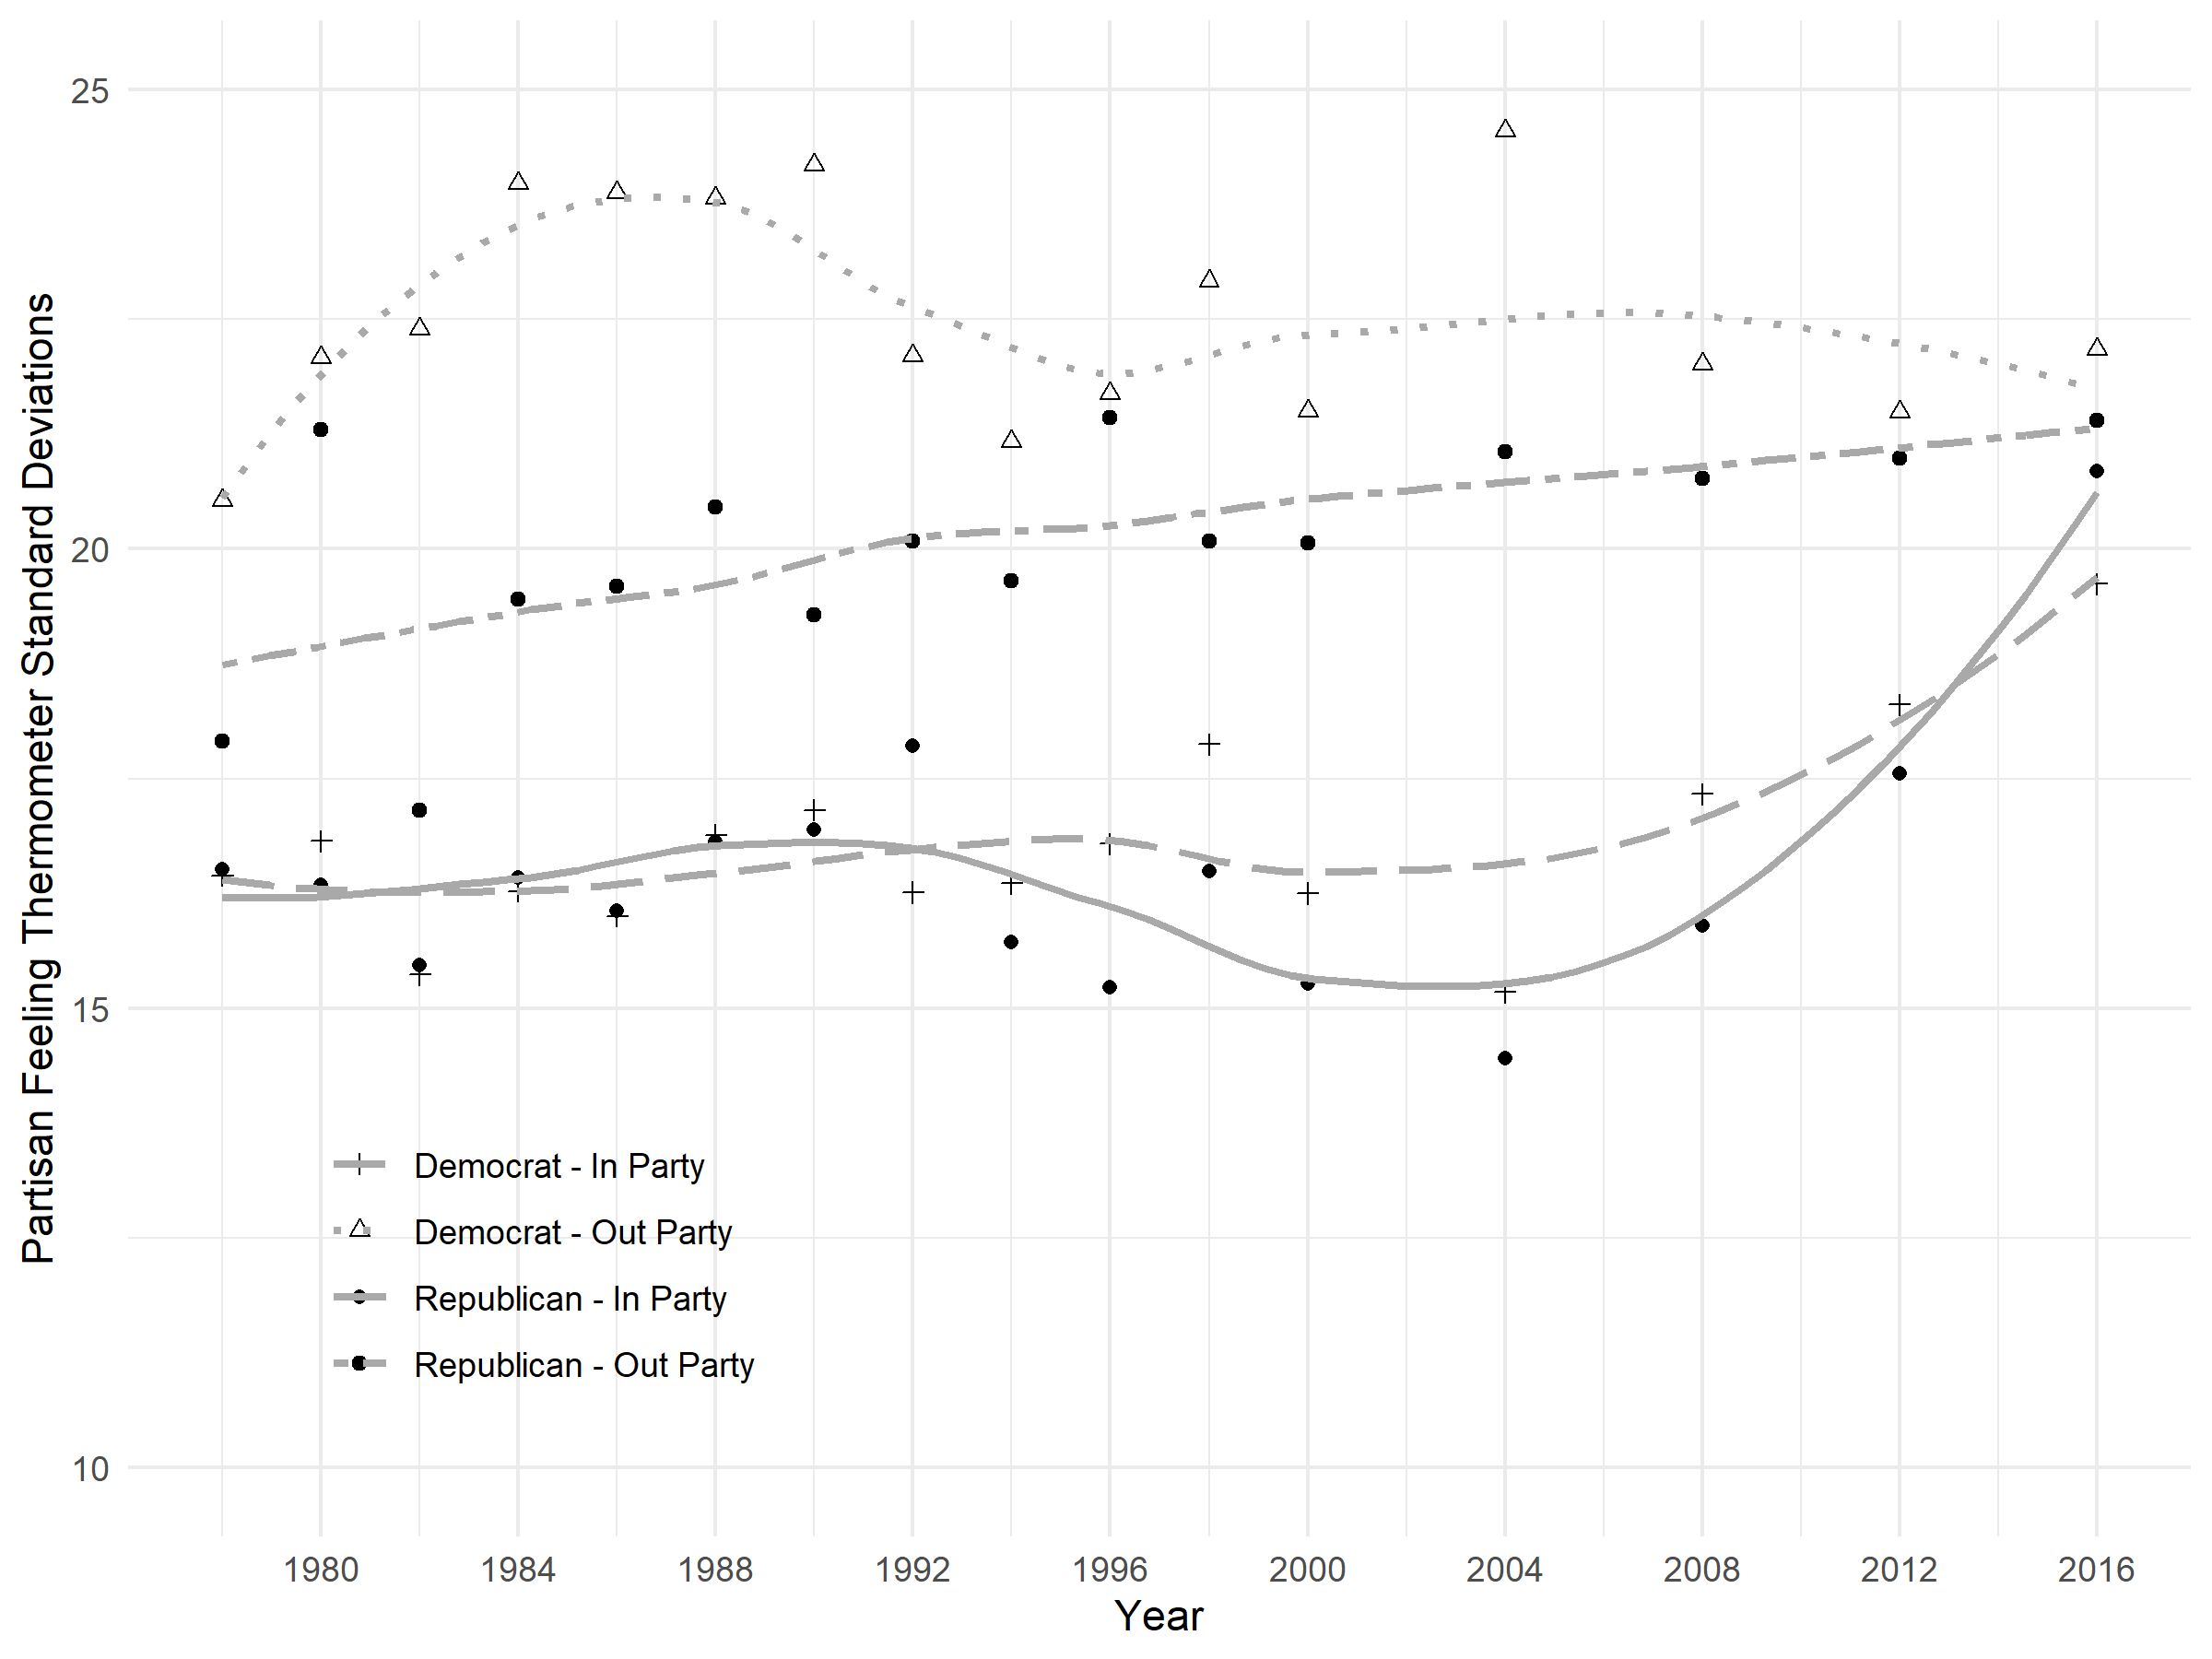
\includegraphics[width=5in]{cdf-sd.png}
%\caption{\label{fig:cdf-sd} \textit{\textbf{Standard Deviation of partisans' in party feeling thermometers, 1978--2016.} After several decades of minimal change, the variation in in-party feeling thermometer ratings increased substantially between 2004 and 2016. This change is robust to both the Fligner-Killeen and Levene's tests of homogeneity of variance.}}
%\end{figure}
%%%%%%
%
%
%
%The changes in variance observed above between 2004 and 2016, as well as 1978-2016 are robust to both the Levene's and Fligner-Killeen tests of homogeneity of variances. These tests evaluate the null hypothesis that the variance of a variable between two samples or groups is equal, and are robust to non-normally distributed data. Each tests rejects the null at $p<.05$ (precise p-values to be reported in the appendix).
%
%%\begin{figure}[H]
%%\center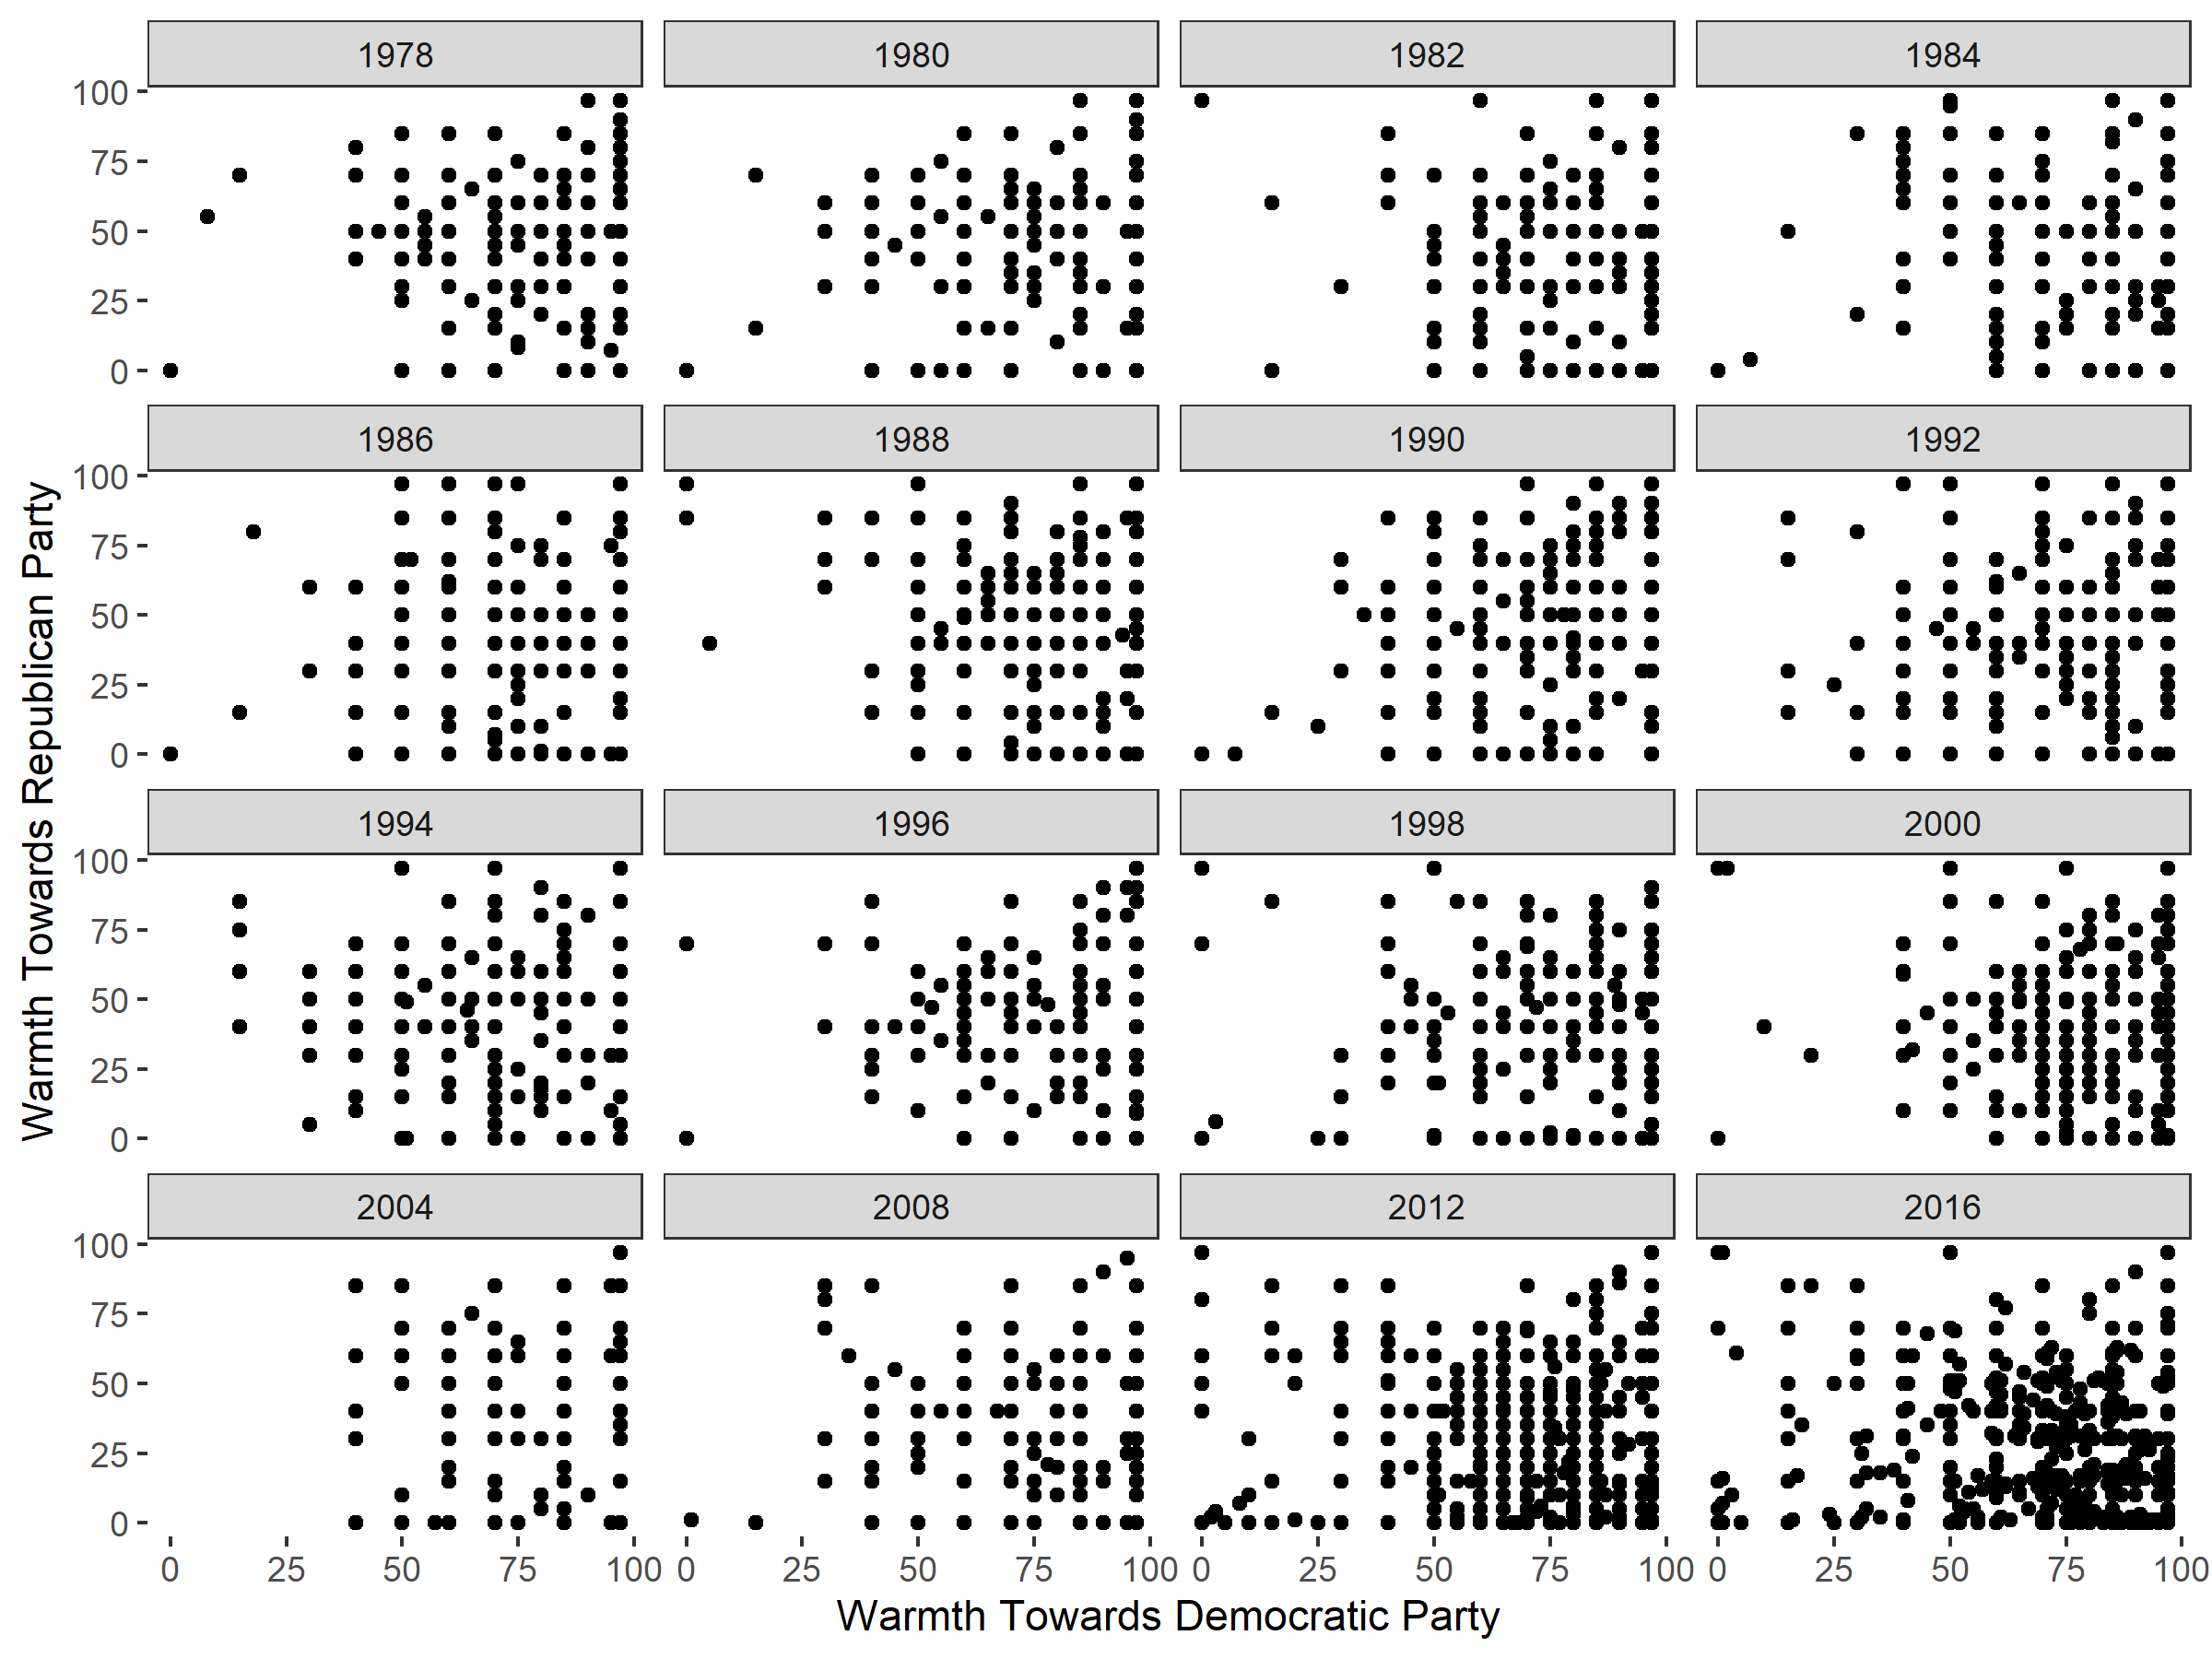
\includegraphics[width=6in]{cdf-scatter-dem.png}
%%\caption{\label{fig:cdf-scatter} \textit{\textbf{Scatterplots of Democrats' feeling thermometer scores toward the Democratic and Republican parties from 1978-2016.} Democrats have gotten more cold towards the Republican Party, but an increasing number are also cold towards \textit{both} parties.}}
%%\end{figure}
%
%%To visualize the variation described above, I scatterplot Democrats' feeling thermometers towards their in-party and out-party, across all available years. Consistent with the theoretical expectation of \cite{iyengar2012affect}, most respondents have clustered in the bottom right of the plot, indicating warmth towards the Democratic party and coldness towards the Republicans. However, in 2012 and 2016, we also see a striking number of respondents in the bottom left, reporting cold affect towards \textit{both} parties. 
%
%%Using a Levene Test---a statistical procedure which evaluates $H_0: \sigma_1 = \sigma_2$, I show that these data are sufficent to reject the null hypothesis stating that Democrat's in-party and out-party feeling thermometers displayed equal variation in 2004 and 2016. The increase in deviation from 2004, when Democrats were (in recent history) most cohesive, to 2016 at their most dispersed is unlikely to be due to chance. We reject the null hypothesis at $p < .001$, as indicated in the tabe below.
%
%%\begin{table}[H]
%%\begin{table}[H]
\centering
\begin{tabular}{>{\raggedright\arraybackslash}p{3cm}>{\raggedleft\arraybackslash}p{3cm}>{\raggedleft\arraybackslash}p{3cm}r}
\toprule
\textbf{ } & \textbf{Df} & \textbf{F value} & \textbf{Pr(>F)}\\
\midrule
group & 1 & 7.423141 & 0.0064838\\
 & 2501 & NA & NA\\
\bottomrule
\end{tabular}
\end{table}
%%\caption{\label{table-levene} \textit{\textbf{Results of a Levene Test on the 2004 and 2016 in-party feeling thermometers of Democrats, which indicates meaningful differences in the deviation of the feeling thermometers}}}
%%\end{table}
%\subsection{A Closer Look At Democrats}
%

%Journalistic accounts of primary elections and their aftermath abound with assertions of internal division and strife within parties after fraught primary election cycles. Democratic primary elections were surprisingly contentious in both 2008 and 2016. In 2008, a particularly brutal primary season spawned the ``Party Unity Means Action" movement (colloquially referred to as the ``Party Unity My Ass" movement) which culminated in an estimated 15-20\% of Clinton supporters voicing their support for John McCain in that year's general election\footnote{\url{https://www.washingtonpost.com/wp-dyn/content/article/2008/06/26/AR2008062604162_pf.html}}.
%
%In 2016 too, primary elections brought to light conflicts between the party's ascendant left-wing and party leadership. These primary divisions seemed to remain salient to engaged voters during the subsequent election for chair of the Democratic National Committee, where Keith Ellison, favored by Sanders supporters lost the race to Obama Secretary of Labor, Tom Perez. Staffers and executives of the 2016 Sanders campaign went on to create groups like \textit{Justice Democrats}, which supports left-leaning candidates in primaries against more centrist Democrats\footnote{Perhaps most notably: \textit{Justice Democrats} supported the campaign of Alexandria Ocasio-Cortez (D-NY), herself a former member of the 2016 Sanders campaign, against former representative Joe Crowley, a high-ranking establishment Democrat.}. 
%
%
%
%
% 
%
%\subsection{Differences in Affect Among Democratic Primary Voters}
%I turn now to subgroup analyses of participants and non-participants in the 2008 and 2016 Democratic primaries. I present data from the three largest categories of ANES respondents in each year. In 2008 these were supporters of Barack Obama and Hillary Clinton; in 2016, Hillary Clinton and Bernie Sanders. In each year non-voters made up a majority of respondents.
%\begin{table}[H]
%\begin{table}[H]
\centering
\begin{tabular}{ll>{\raggedleft\arraybackslash}p{3cm}>{\raggedleft\arraybackslash}p{3cm}>{\raggedleft\arraybackslash}p{3cm}>{}p{3cm}>{}p{3cm}>{}p{3cm}}
\toprule
\textbf{Year} & \textbf{Vote Choice} & \textbf{Net Partisan Affect} & \textbf{Dem Affect} & \textbf{Rep Affect}\\
\midrule
2008 & Didn't Vote & 47.43 & 78.55 & 31.76\\
2008 & Hillary Clinton & 48.37 & 76.51 & 28.14\\
2008 & Barack Obama & 53.63 & 80.40 & 26.77\\
2016 & Didn't Vote & 45.80 & 71.99 & 28.60\\
2016 & Hillary Clinton & 60.19 & 82.62 & 22.48\\
\addlinespace
2016 & Bernie Sanders & 48.34 & 67.70 & 21.45\\
\bottomrule
\end{tabular}
\end{table}
%\caption{\label{table} \textit{\textbf{In-party, out-party, and net-affect of supporters of major Democratic primary candidates.} Other candidates have been excluded due to very low sample size. These data are filtered by party-ID; all respondents are Democrats.}}
%\end{table}
%In 2008 Democrats were largely warm to the party, with averaged feeling thermometers toward their own party in the high 70s or low 80s, in the case of Obama supporters. Clinton voters profess the lowest NPA (identical to that of Bernie voters' in 2016). Consistent with the observed increase in variation, Clinton and Obama voters' net party affects were more similar than those of Clinton and Sanders supporters in 2016.
%
%As expected, affect toward toward republicans dropped across voters and non-voters between 2008 and 2016.  That year, Clinton voters' NPA was substantially higher than that of any other group, and their warmth toward the Democratic party is the highest of all six groups. Bernie voters' net affect is much lower, at about 48. Examining affect toward the Democratic and Republican parties individually, it is clear that Bernie voters' low NPA is the product of coldness towards the Democratic party on the part of Sanders supporters, rather than any particular warmth towards the Republicans. Bernie supporters reported both the lowest in-party thermometer rating (15 points lower than Clinton supporters in 2016) and the lowest out-party score, a point colder towards Republicans than Clinton voters.
%
%\begin{figure}[H]
%\center
\includegraphics[width=6in]{primary-scatter.png}
%\caption{\label{fig:primary-scatter} \textit{\textbf{Scatterplots of 2008 and 2016 Democratic primary voters Democrat and Republican feeling thermometers.} Mean Democratic feeling thermometer for all groups in each year indicated by vertical line.}}
%\end{figure}
%
%When viewing scatterplots of the data presented in table 1, the differences between each group are immediately apparent---particularly in 2016. In 2008, Obama supporters were uniformly warm to the Democratic Party, not a single respondent reported a feeling thermometer below 50. Hillary supporters skewed somewhat colder, but were still generally warm to the Democrats. 
%
%Turning to 2016, Most Hillary supporters were overwhelmingly warm to their party. Bernie voters, on the other hand, are much more ambivalent toward their party. Sanders supporters more closely resemble non-voters from 2016 than any other group in the data. They were less likely than their co-partisans to rate their in-party affect a full 100 and not a single one of those who did rated Republicans above a 25.
%
%Democrats' in-party affect is more heterogenous than has been suggested by existing literature. Variation in Democrats' in-party affect has been increasing since 2004, while mean in-party affect has remained relatively constant, indicating that increasing numbers of Democrats are quite warm to their party, while other groups are lukewarm, or even cold. It is more appropriate to say that Democrats' in-party affect has polarized somewhat, than that to simply claim that it has remained stable.
%
%%
%%The data presented above suggest a more complicated picture of Democrats' affect than annual averages would suggest, more suggestive of modest polarization than the stability of opinion insinuated by simple annual averages. It is not that Democrats on the whole feel the same way about the party today as they did in the 1980s, but that some have grown warmer to the party while other have grown colder. In short, Democrats are polarizing---albeit modestly---in their feelings of their own party.
%
%
% A potential explanation for these findings is that losing a primary election causes supporters of the losing candidates to dislike the party. Hillary supporters were most cold toward the party in 2008, as were Bernie supporters in 2016. It is also possible that some primary candidates bring new voters into the party, who may not be as friendly towards the organization as existing partisans. This hypothesis seems particularly likely in the case of Sanders in 2016, who did particularly well with those identifying as leaning independents. These hypotheses could be evaluated using panel data to track respondents' changes in partisanship over time.
%
%Finally, the role of ideology in primary vote choice and affect should also be further investigated. While \cite{iyengar2012affect} argue that ideology plays only a minor role in shaping peoples' affective responses, it may be more prevalent among primary voters, who are particularly engaged and attuned to politics \citep{iyengar2012affect}. The affective cleavages between opposing primary voters may be the product of substantive differences on the issues. It is also possible that primary voters chosen candidate functions as an element of their political identity. Possessing a social identity necessitates an in-group and an out-group \citep{brewer2001many}. If a Sanders supporter thinks of their in-group as other Sanders supporters rather than the party writ-large, they may be predisposed to see the party (whose elites overwhelmingly supported Clinton) as a hostile out-group. 
%
%
% Table created by stargazer v.5.2.2 by Marek Hlavac, Harvard University. E-mail: hlavac at fas.harvard.edu
% Date and time: Tue, Apr 21, 2020 - 3:25:30 AM
% Requires LaTeX packages: dcolumn 
\begin{table}[H] \centering 
  \caption{Replicating ISL's Models} 
  \label{} 
\begin{tabular}{@{\extracolsep{-5pt}}lD{.}{.}{-2} D{.}{.}{-2} D{.}{.}{-2} D{.}{.}{-2} } 
\\[-1.8ex]\hline 
\hline \\[-1.8ex] 
 & \multicolumn{4}{c}{Covariates of Net Partisan Affect} \\ 
\cline{2-5} 
\\[-1.8ex] & \multicolumn{2}{c}{1988} & \multicolumn{2}{c}{2004} \\ 
 & \multicolumn{1}{c}{Democrats} & \multicolumn{1}{c}{Republicans} & \multicolumn{1}{c}{Democrats} & \multicolumn{1}{c}{Republicans} \\ 
\\[-1.8ex] & \multicolumn{1}{c}{(1)} & \multicolumn{1}{c}{(2)} & \multicolumn{1}{c}{(3)} & \multicolumn{1}{c}{(4)}\\ 
\hline \\[-1.8ex] 
 Cultural Attitudes & -0.05 & 0.04 & 0.05 & 0.04 \\ 
  & (0.04) & (0.03) & (0.05) & (0.04) \\ 
  & & & & \\ 
 Economic Attitudes & 0.16^{***} & 0.18^{***} & 0.15^{**} & 0.18^{***} \\ 
  & (0.05) & (0.05) & (0.06) & (0.06) \\ 
  & & & & \\ 
 Strong Partisan & 0.19^{***} & 0.18^{***} & 0.27^{***} & 0.24^{***} \\ 
  & (0.02) & (0.02) & (0.02) & (0.02) \\ 
  & & & & \\ 
 Political Knowledge & 0.06 & 0.05 & 0.09^{*} & 0.11^{*} \\ 
  & (0.04) & (0.04) & (0.05) & (0.06) \\ 
  & & & & \\ 
 Gender: Female & 0.01 & -0.01 & 0.04 & 0.01 \\ 
  & (0.02) & (0.02) & (0.02) & (0.02) \\ 
  & & & & \\ 
 Region: South & -0.04^{*} & 0.06^{***} & 0.04^{*} & 0.05^{**} \\ 
  & (0.02) & (0.02) & (0.02) & (0.02) \\ 
  & & & & \\ 
 Race: White & -0.04^{**} & -0.001 & 0.003 & 0.02 \\ 
  & (0.02) & (0.03) & (0.02) & (0.03) \\ 
  & & & & \\ 
 High School & -0.05 & -0.01 & -0.17^{**} & 0.06 \\ 
  & (0.03) & (0.04) & (0.07) & (0.09) \\ 
  & & & & \\ 
 Some College & -0.04 & -0.01 & -0.16^{**} & 0.04 \\ 
  & (0.04) & (0.04) & (0.07) & (0.09) \\ 
  & & & & \\ 
 College or Advanced Degree & -0.03 & -0.02 & -0.16^{**} & 0.02 \\ 
  & (0.04) & (0.04) & (0.07) & (0.09) \\ 
  & & & & \\ 
 Constant & 0.24^{***} & 0.13^{**} & 0.21^{**} & 0.01 \\ 
  & (0.06) & (0.05) & (0.09) & (0.09) \\ 
  & & & & \\ 
\hline \\[-1.8ex] 
Observations & \multicolumn{1}{c}{891} & \multicolumn{1}{c}{778} & \multicolumn{1}{c}{556} & \multicolumn{1}{c}{473} \\ 
Adjusted R$^{2}$ & \multicolumn{1}{c}{0.14} & \multicolumn{1}{c}{0.16} & \multicolumn{1}{c}{0.25} & \multicolumn{1}{c}{0.26} \\ 
\hline 
\hline \\[-1.8ex] 
\textit{Note:}  & \multicolumn{4}{r}{$^{*}$p$<$0.1; $^{**}$p$<$0.05; $^{***}$p$<$0.01} \\ 
\end{tabular} 
\end{table} 

%
%% Table created by stargazer v.5.2.2 by Marek Hlavac, Harvard University. E-mail: hlavac at fas.harvard.edu
%% Date and time: Mon, Apr 20, 2020 - 3:55:54 PM
%\subsubsection{Unit of Analysis}

%\citeauthor{iyengar2012affect} use individual level attitudinal data to make inferences about the state of the broader population. Their primary hypothesis is that the United States exists in an increasingly affective polarized state---a condition which is only possible to achieve through the individual attitudes of many individuals. Referring to the DAG presented in \textit{Figure \ref{fig:dag}}, we see that polarization is wholly dependent on individual out-party animus. In this case it is perfectly legitimate to draw mass level inferences from individual level data.

%\subsubsection{Manipulability \& Randomization}

%Party ID is difficult to manipulate in an observational study. It is conceivable that an experimental design could assign participants a particular party ID in the limited context of that experiment, but given the importance of individuals’ actual party ID there would be reason to doubt the external validity of such a study. 

%Media exposure can be more easily manipulated in an experimental setting, as in \citet{mutz2007effects}, but the external validity of such experiments is questionable, given the differences between media consumption in the laboratory and in more complex information environments. Fortunately, the opportunity to conduct a natural experiment outside of the laboratory environment exists.

%Iyengar et al use residence in a ``battleground state"\footnote{Defined by the authors as ``States with the two parties’ vote difference of less than 5 percent in the 2000 elections...FL, IA, MO, MN, NH, NM, NV, OH, OR, PA, and WI".} as the exposure variable in their regression to capture the effect of hostile media on partisans' affect (p. 424). Greater causal leverage could be gained over the effect of media by instead conducting a natural experiment using a Geographic Regression Discontinuity (GRD) design. Campaign ads are purchased and distributed in ``Designated Market Areas (DMAs)", collections of counties in which a television ad is shown. These DMAs may extend across multiple states \citep{keele2015geographic}. In other words: residents of a non-battleground state $A$ may reside in a DMA which largely services a battleground state $B$. Residents of the DMA in state $A$ will be exposed to the ads targeting state $B$. Residents of state $A$ living outside the DMA will not be exposed to battleground ads.

%In such a GRD design, state $A$ counties in state $B$'s DMA are considered the treatment group, while state $A$ counties \textit{adjacent} to the DMA are considered the control. While individuals likely self-select into states, it is unlikely that residents self-select into particular DMAs \textit{within} those states. Extant scholarship has exploited this as-if random assignment in the study of media and voter turnout \cite{krasno2008televised, huber2007identifying}.





%Designated Media Exposure



%\subsubsection{Implicit Counterfactuals}
%The implicit counterfactual, a condition of weak partisan identity, is not necessarily unrealistic but is \textit{unlikely}. The salience of partisan identity appears to be at a historical high, and the trend does not appear poised to level out any time soon. Still, some researchers have demonstrated experimental interventions which seem to decrease the importance of party ID to participants (Levendusky, Forthcoming). Additionally, both major parties seem to be undergoing a period of increased ideological heterogeneity, with the left and moderate wings of the Democratic party seemingly ascendant and the embrace of Trump by many (but not all) elites in the Republican party. Scholars have argued that internal ideological heterogeneity was a sufficient condition for the (relatively) low salience of party ID through much of the 20th Century \citep{rohde1991parties}; as such, there is reason not to entirely discount the possibility of a return to an era of relatively weak party ID.

%\subsubsection{SUTVA}
%The Stable Unit Treatment Value Assumption (SUTVA) is the assumption that one individual receiving (or not) the treatment condition does not not affect the outcome in other individuals in the study---the effect of $x$ on $i_1$ is the same, regardless of if (or how) individuals $i_2 \ldots i_n$ received the treatment \citep[p. 48]{morgan2015counterfactuals}. 
%SUTVA is violated in this model, with the potential for spillover effects between partisans. While posing problems for causal inference, this SUTVA violation is intrinsic to the study of polarization. Polarization, by definition, implies an in-group and an outgroup; the compositions of which influence the attitudes of the other. 

%The outcome we are interested in is the social distance between individuals $d_n$ and $r_n$ in groups $D$ and $R$. We can expect this effect to vary based on the treatment homogeneity of $D$ and $R$. In other words, the effect produced by one individual’s partisan identity can depend on the identities and the strength of those around her. For a group identity to be salient (and therefore to produce a powerful effect on social distance towards an outgroup) we would expect to find heterogeneity in the outgroup and homogeneity in the ingroup \citep{rohde1991parties}. As noted by the authors of this study (and authors of more recent work) the observed increase in affective polarization has been concomitant with elite-level partisan sorting over the 20th and 21st centuries. 

%\subsubsection{Endogeneity \& Confounders}


%While the \textit{central} hypothesis of this study is largely descriptive, the DAG describing the data-generating process of \citeauthor{iyengar2012affect} is complex---containing several other potential problem areas. The DAG confusion arises because several of the nodes are both exposure and outcome variables. For example, in \textbf{\textit{H2}} party ID is the exposure variable, whereas it is an outcome in \textbf{\textit{H3}}. The authors' theory holds that the media affects affective polarization \textit{only} through its effect on party ID (p. 407), yet the party ID variable is included in the regression equation for media exposure on partisan affect, suggesting possible over control bias.

%There are two possibilities:
%\begin{enumerate}
%\item The theory is correct, and the effect of media has been underestimated due to controlling for a node  in the middle of a causal path \citep{elwert2014endogenous}.
%\item The theory needs to be amended; media effects partisan affect in ways that are not predicated on an increased sense of party ID.
%\end{enumerate}
%In addition to this concern, there is the possibility of over control bias when evaluating the effect of policy preferences on affect, as policy preferences are often endogenous to party ID \citep{druckman2013elite}\footnote{This is also acknowledged in the footnotes on page 422 of \citeauthor{iyengar2012affect}.} This case is not alarming however, as party ID was not included as a variable when regressing affect on policy preferences. While the authors' articulation of their causal claim is problematic, their core descriptive claim (that the United States has increasingly affectively polarized since the mid-\nth{20} century) is unaffected by these problems.

\end{document}

%